\documentclass{if-beamer}

% --------------------------------------------------- %
%                  Presentation info	              %
% --------------------------------------------------- %
\title[Projeto -- Etapa 3]{Arquitetura HIL para teste de sistemas embarcados como \textit{vehicle interface} de veículos autônomos baseados no Autoware}
\subtitle{Projeto -- Etapa 3}

\author[Gabriel Toffanetto]{\texorpdfstring
	{Gabriel Toffanetto França da Rocha 
		\\ \vspace{1mm} 
		\small{\href{mailto:g289320@dac.unicamp.br}{g289320@dac.unicamp.br}}
	}
	{Gabriel Toffanetto França da Rocha}
}

\institute[LMA/FEM/Unicamp]{\small{Professor Dr. Rodrigo Moreira Bacurau
  \\ \vspace{2mm}
  IM420X -- Projeto de Sistemas Embarcados de Tempo Real
  \\ \vspace{4mm}
  Faculdade de Engenharia Mecânica
  \\ \vspace{1mm}
  Universidade Estadual de Campinas}
}

\date{12 de novembro de 2024}

\logo{
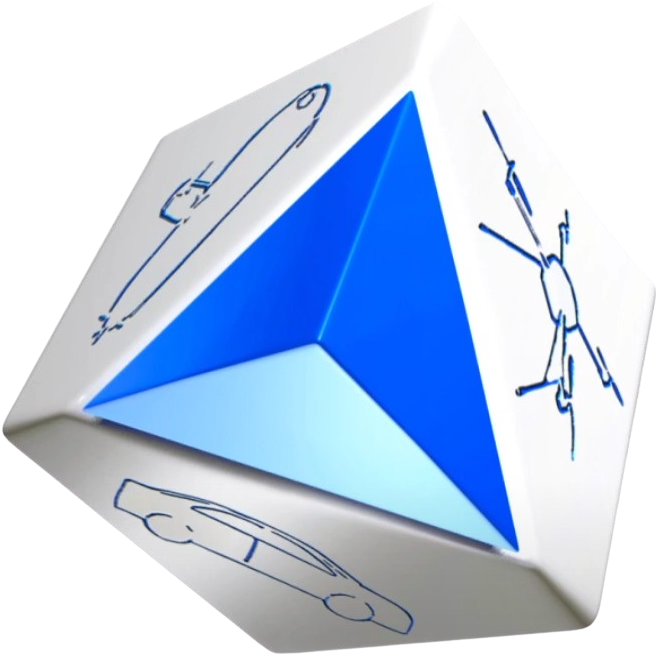
\includegraphics[width=1.2cm]{img/core/Logo_LMA_icon.png}
}


\subject{IM420X - Projeto final: Etapa 2} % metadata

\graphicspath{{img/}}

\setbeamertemplate{caption}[numbered]

\newcolumntype{b}{>{\columncolor{white}}c}


\hypersetup{pdfpagemode=FullScreen}


% --------------------------------------------------- %
%                    Title + Schedule                 %
% --------------------------------------------------- %

\begin{document}

\begin{frame}
  \titlepage
\end{frame}

\begin{frame}{Agenda}
  \tableofcontents
\end{frame}

% --------------------------------------------------- %
%                      Presentation                   %
% --------------------------------------------------- %

\section{Introdução}

\begin{frame}{Proposta}
	
	\begin{columns}
		
		\begin{column}{0.6\textwidth}
			
				\begin{figure}[H]
				\centering
				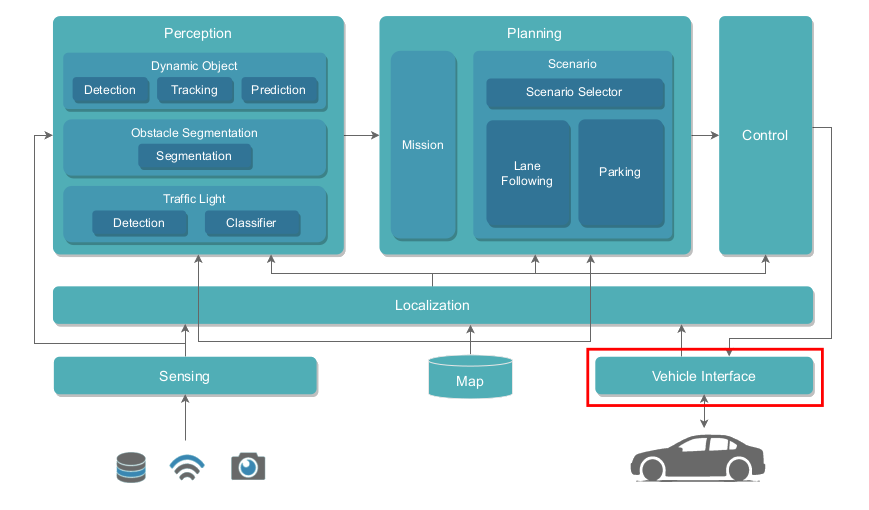
\includegraphics[width=\linewidth]{img/architecture.png}
				\caption{Escopo do projeto na arquitetura Autoware.}
				\label{fig:architecture}
			\end{figure}
			
		\end{column}
		
		\hspace{-0.5cm}
		
		\begin{column}{0.45\textwidth}
			
				\begin{figure}[H]
				\centering
				\includegraphics[width=\linewidth]{img/architecture_HIL}
				\caption{Arquitetura de teste do \textit{hardware}.}
				\label{fig:architecture_HIL}
			\end{figure}
			
		\end{column}
		
	\end{columns}
	
\end{frame}

\section[Sistema embarcado]{Atualizações no sistema embarcado}

\begin{frame}{Diagrama de blocos}
	
	\begin{block}{}
		
		\begin{itemize}
			\item Sobrecarga do micro-ROS para controle e tráfego dos dados do simulador;
			\item Aproximação que leva à \textit{overhead} comparado com a arquitetura real.
			
		\end{itemize}
		
	\end{block}
	
	\begin{figure}[H]
		\centering
		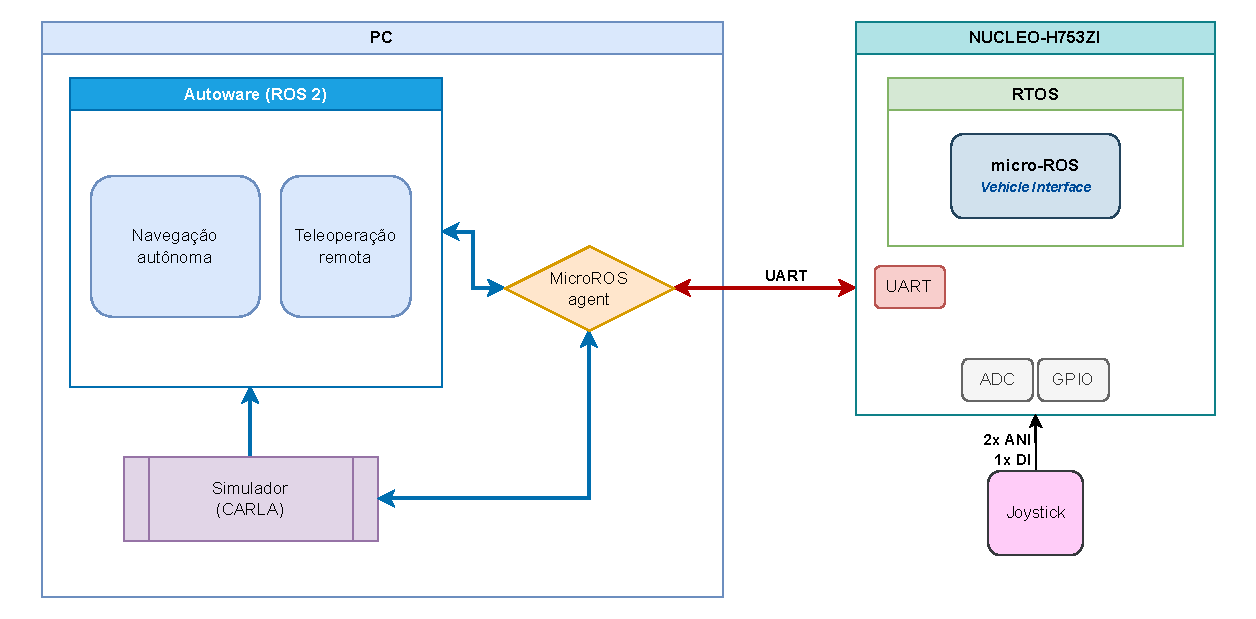
\includegraphics[width=0.75\linewidth]{block_diagram_old}
		\caption{Diagrama de blocos atualizado.}
		\label{fig:block_diagram_old}
	\end{figure}
	
\end{frame}

\begin{frame}{Diagrama de blocos}
	
	\begin{figure}[H]
		\centering
		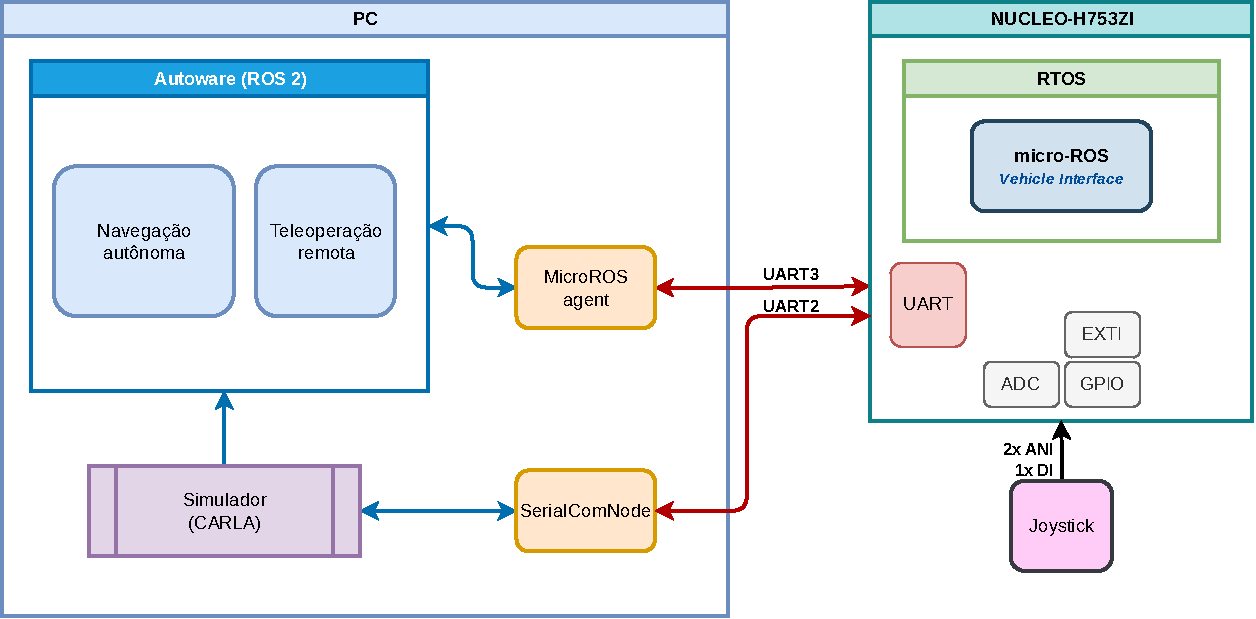
\includegraphics[width=0.9\linewidth]{block_diagram}
		\caption{Diagrama de blocos atualizado.}
		\label{fig:block_diagram}
	\end{figure}

\end{frame}

\begin{frame}{Diagrama de tarefas}
	
	\begin{figure}[H]
		\centering
		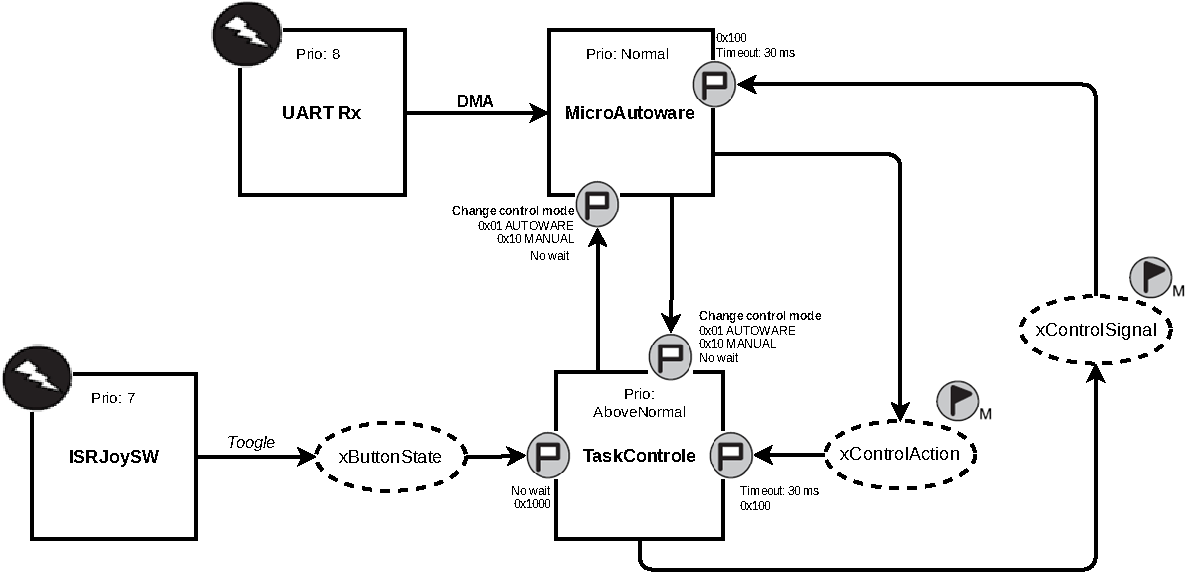
\includegraphics[width=0.95\linewidth]{system_diagram_old}
		\caption{Diagrama de tarefas antigo.}
		\label{fig:system_diagram_old}
	\end{figure}
	
\end{frame}

\begin{frame}{Diagrama de tarefas}
	
	\begin{figure}[H]
		\centering
		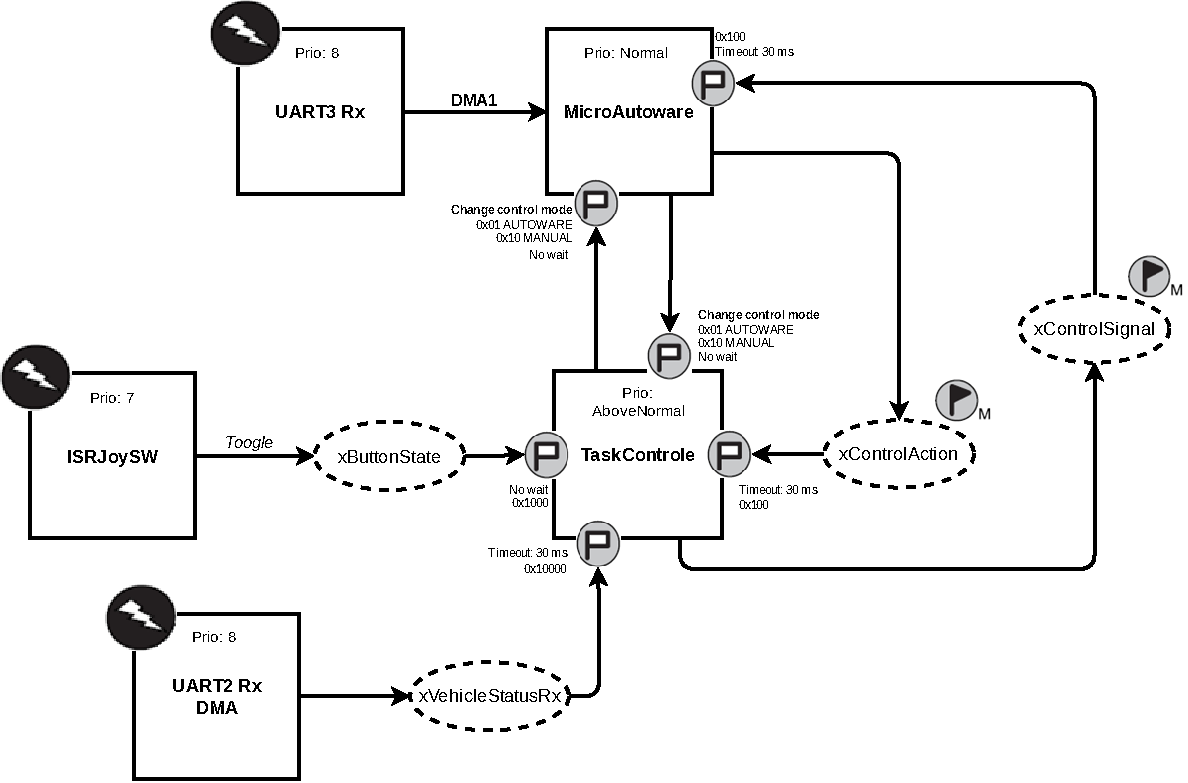
\includegraphics[width=0.75\linewidth]{system_diagram}
		\caption{Diagrama de tarefas atualizado.}
		\label{fig:system_diagram}
	\end{figure}

\end{frame}

\begin{frame}{Comunicação com o simulador}
	
	\begin{columns}
		
		\begin{column}{0.435\textwidth}
			
			\begin{block}{Sistema embarcado $\longrightarrow$ CARLA}
				
				\begin{itemize}
					\item \texttt{float fSteeringAngle;}
					\item \texttt{float fSteeringVelocity;}
					\item \texttt{float fSpeed;}
					\item \texttt{float fAcceleration;}
					\item \texttt{float fJerk;}	
					\item \texttt{unsigned char ucControlMode;}					
				\end{itemize}
				
			\end{block}
			
		\end{column}
		
		\begin{column}{0.435\textwidth}
			
			\begin{block}{CARLA $\longrightarrow$ Sistema embarcado }
				
				\begin{itemize}
					\item \texttt{float fLongSpeed;}
					\item \texttt{float fLatSpeed;}
					\item \texttt{float fHeadingRate;}
					\item \texttt{float fSteeringStatus;}
					
				\end{itemize}
			
				
				
			\end{block}
			
		\end{column}
		
	\end{columns}

	\begin{block}{}
		
		\textbf{Padrão de Mensagem:} Sistema embarcado $\longrightarrow$ CARLA
		
		\begin{itemize}
			\item \textbf{\#S}\texttt{\%c\%c\%c\%c}\textbf{W}\texttt{\%c\%c\%c\%c}\textbf{V}\texttt{\%c\%c\%c\%c}\textbf{A}\texttt{\%c\%c\%c\%c}\textbf{J}\texttt{\%c\%c\%c\%c}\textbf{M}\texttt{\%c}\textbf{\$}
			\item 30 bytes
			
		\end{itemize}
		
		\textbf{Padro de Mensagem:} CARLA $\longrightarrow$ Sistema embarcado
		\begin{itemize}
			\item \textbf{\#A}\texttt{\%c\%c\%c\%c}\textbf{B}\texttt{\%c\%c\%c\%c}\textbf{C}\texttt{\%c\%c\%c\%c}\textbf{D}\texttt{\%c\%c\%c\%c}\textbf{\$}
			\item 22 bytes
			
		\end{itemize}
		
	\end{block}
	
\end{frame}

\begin{frame}{Máquinas de estados de comunicação}
	
	\begin{figure}[H]
		\centering
		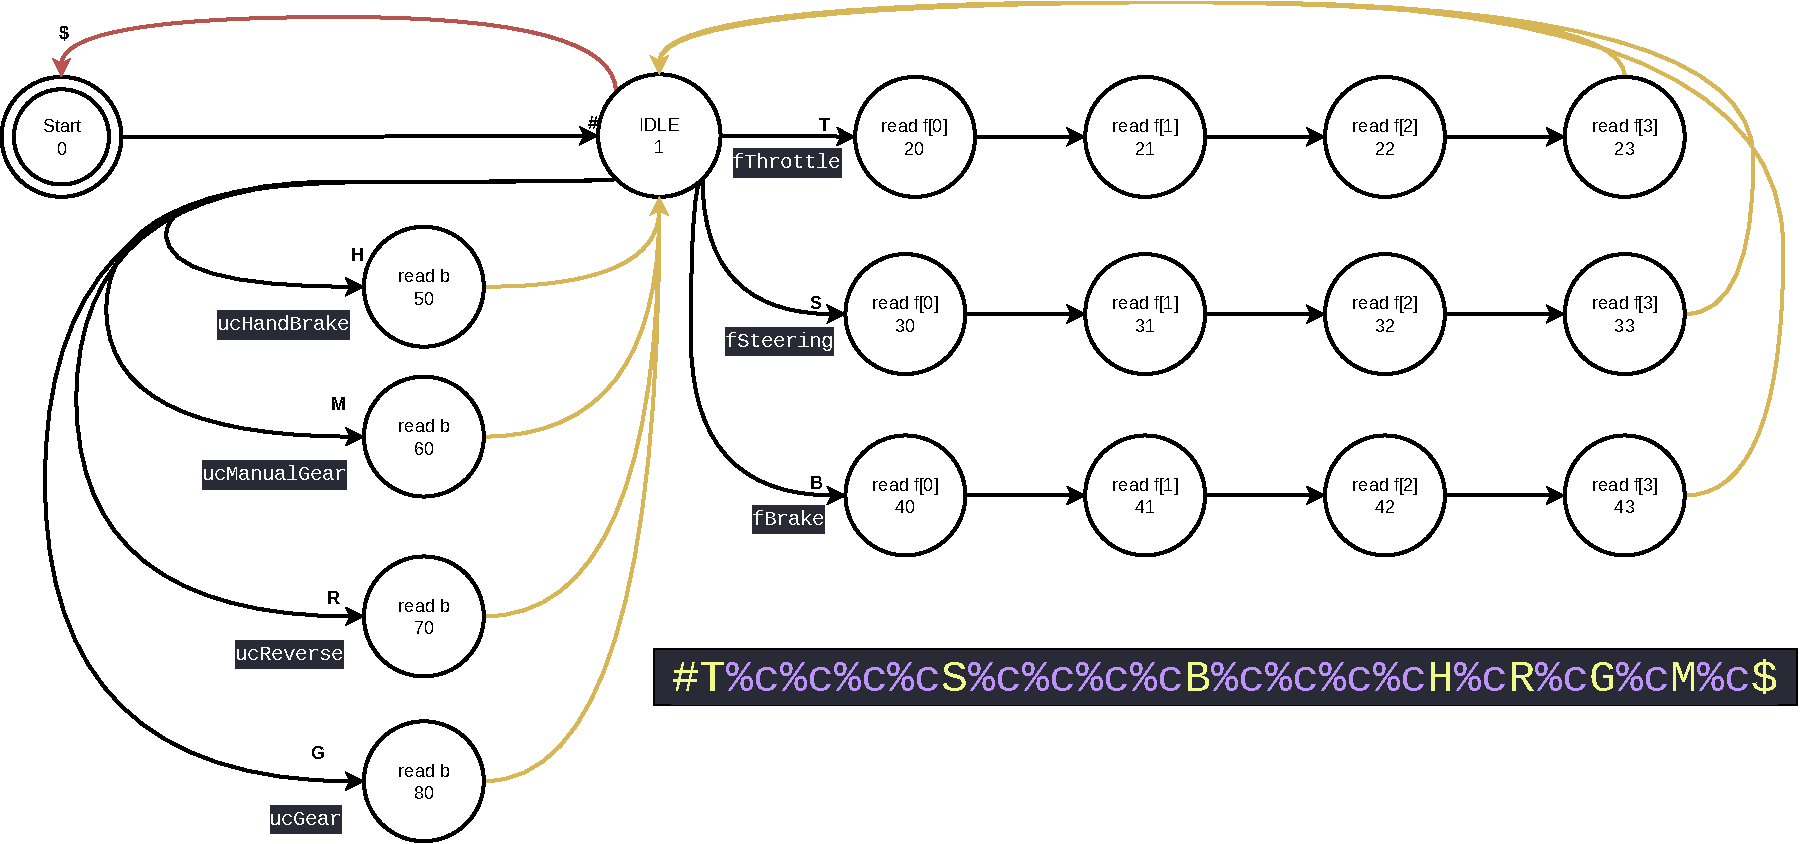
\includegraphics[width=0.8\linewidth]{sm_uc_2_carla}
		\caption{Maquina de estados da comunicação sistema embarcado $\longrightarrow$ CARLA (\texttt{CarlaSerialBridgeNode}).}
		\label{fig:sm_uc_2_carla}
	\end{figure}
	
\end{frame}

\begin{frame}{Máquinas de estados de comunicação}
	
	\begin{figure}[H]
		\centering
		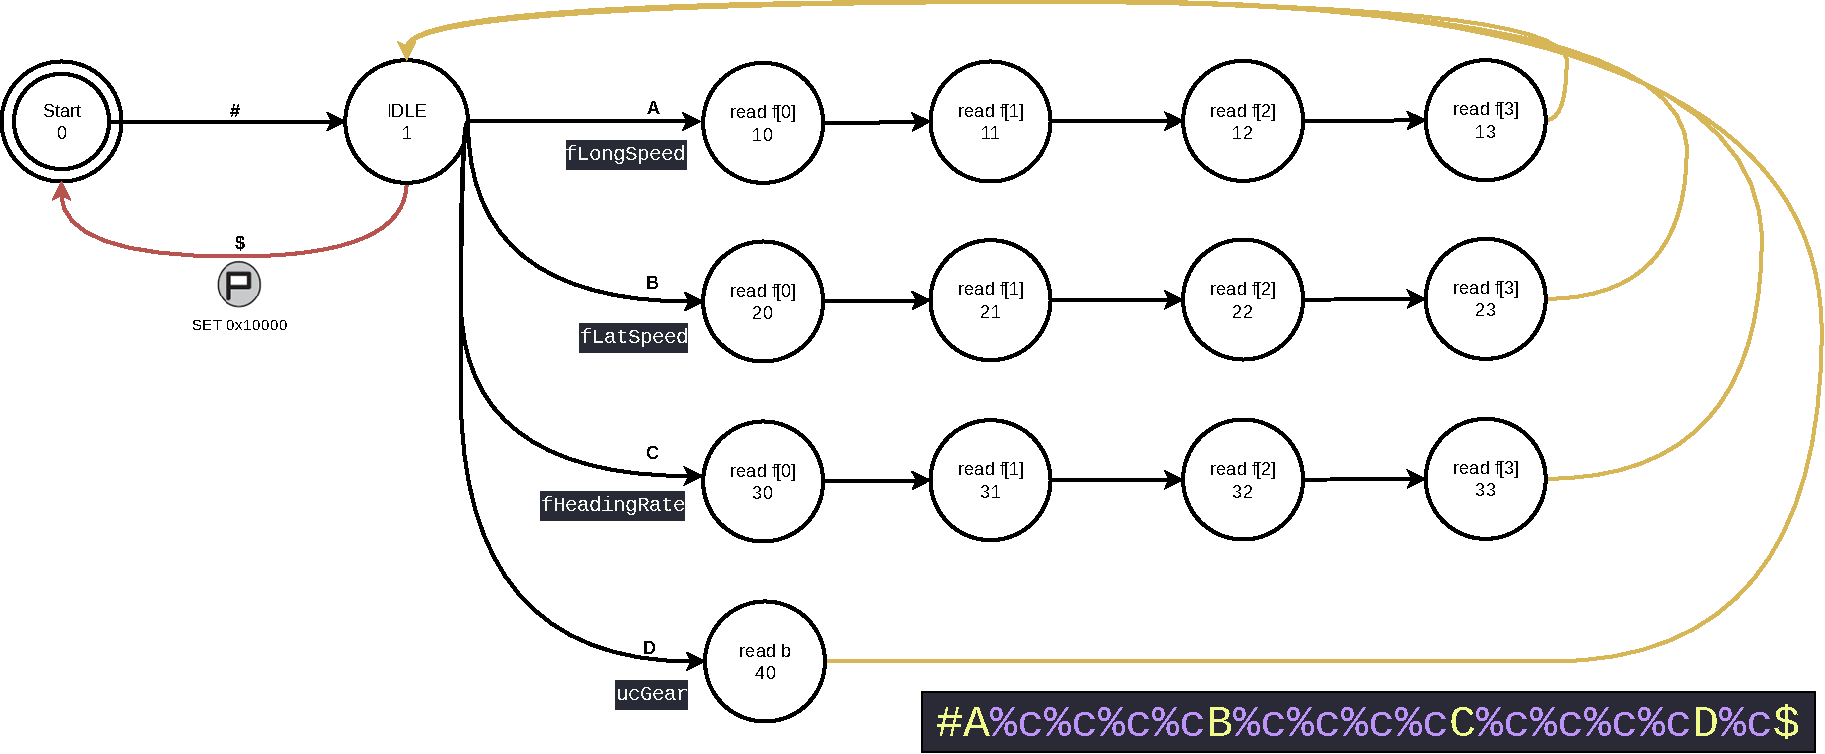
\includegraphics[width=\linewidth]{sm_carla_2_uc}
		\caption{Maquina de estados da comunicação CARLA $\longrightarrow$ sistema embarcado (\texttt{HAL\_UART\_RxCpltCallback()}).}
		\label{fig:sm_carla_2_uc}
	\end{figure}

\end{frame}


\section{Testes dos módulos}

\begin{frame}{Montagem do \textit{hardware}}
	
	\begin{figure}[H]
		\centering
		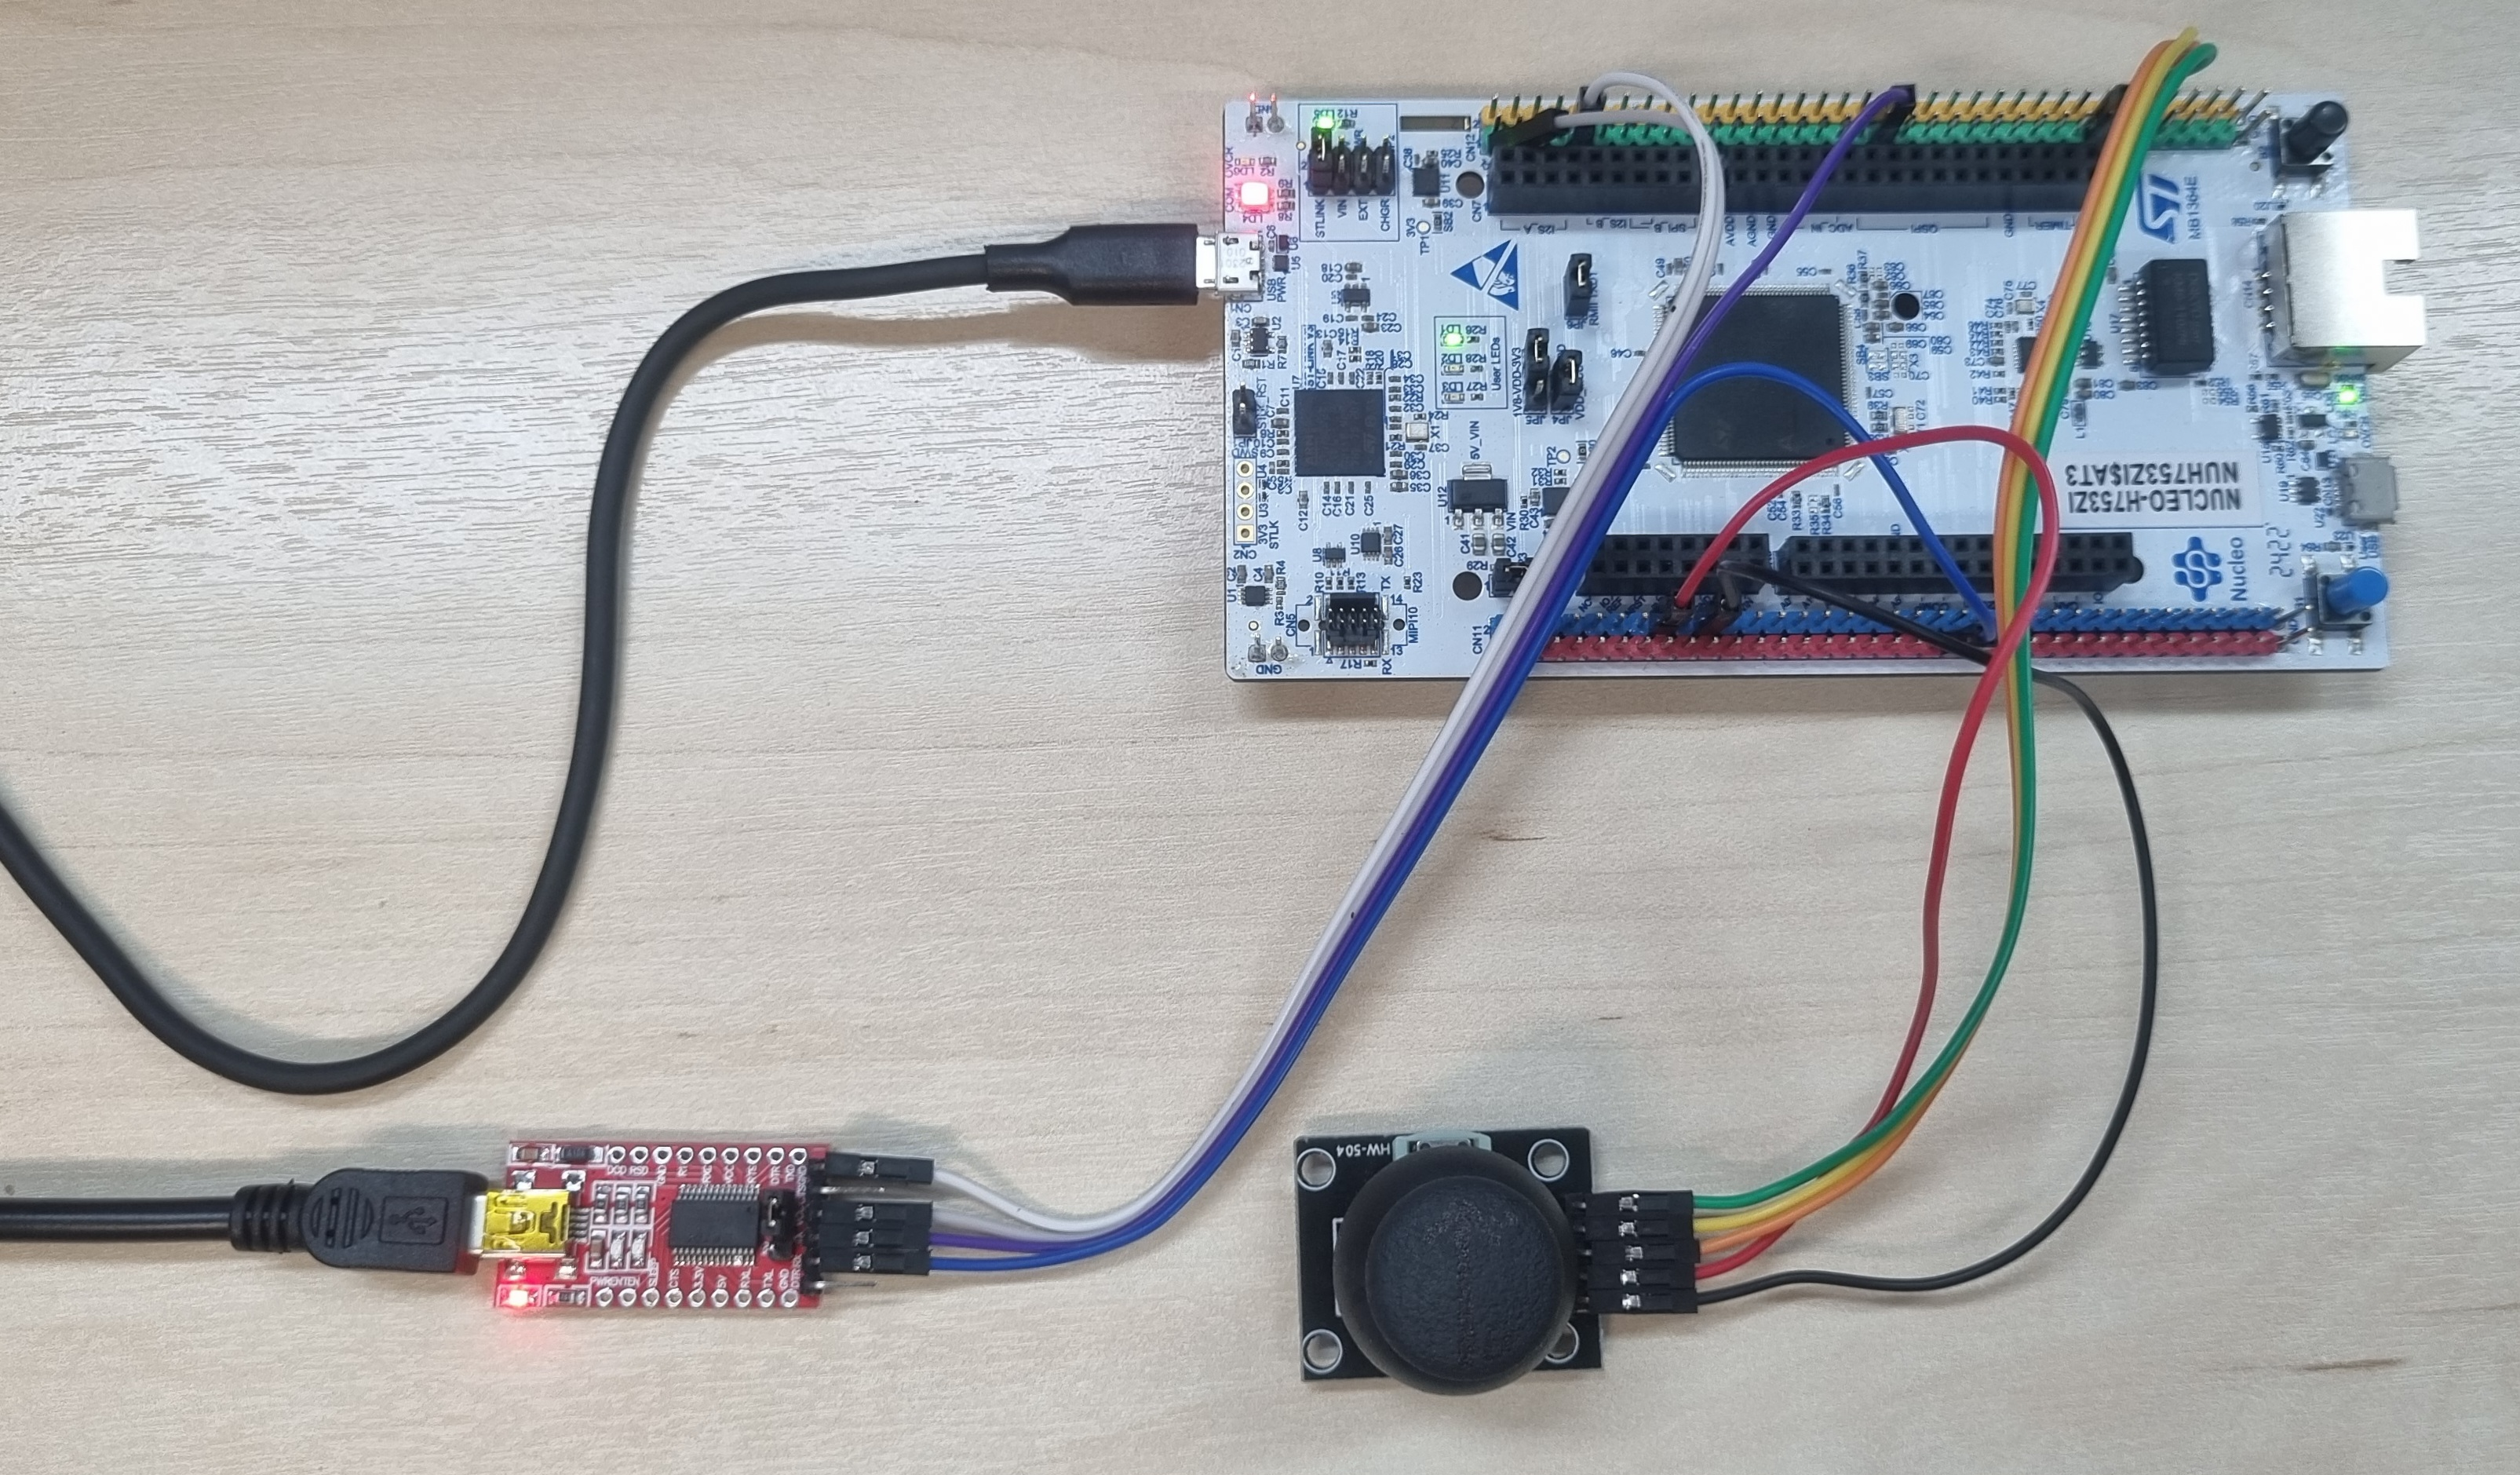
\includegraphics[width=0.8\linewidth]{montagem}
		\caption{Montagem física dos componentes utilizados.}
		\label{fig:somevideo}
	\end{figure}
	
	
	
\end{frame}

\begin{frame}{Leitura do \textit{Joystick} + Comunicação serial com o \texttt{CarlaSerialBridge}}
	
	\begin{figure}[H]
		\centering
		\movie[width=\textwidth,height=0.422\textwidth,poster,autostart,loop]{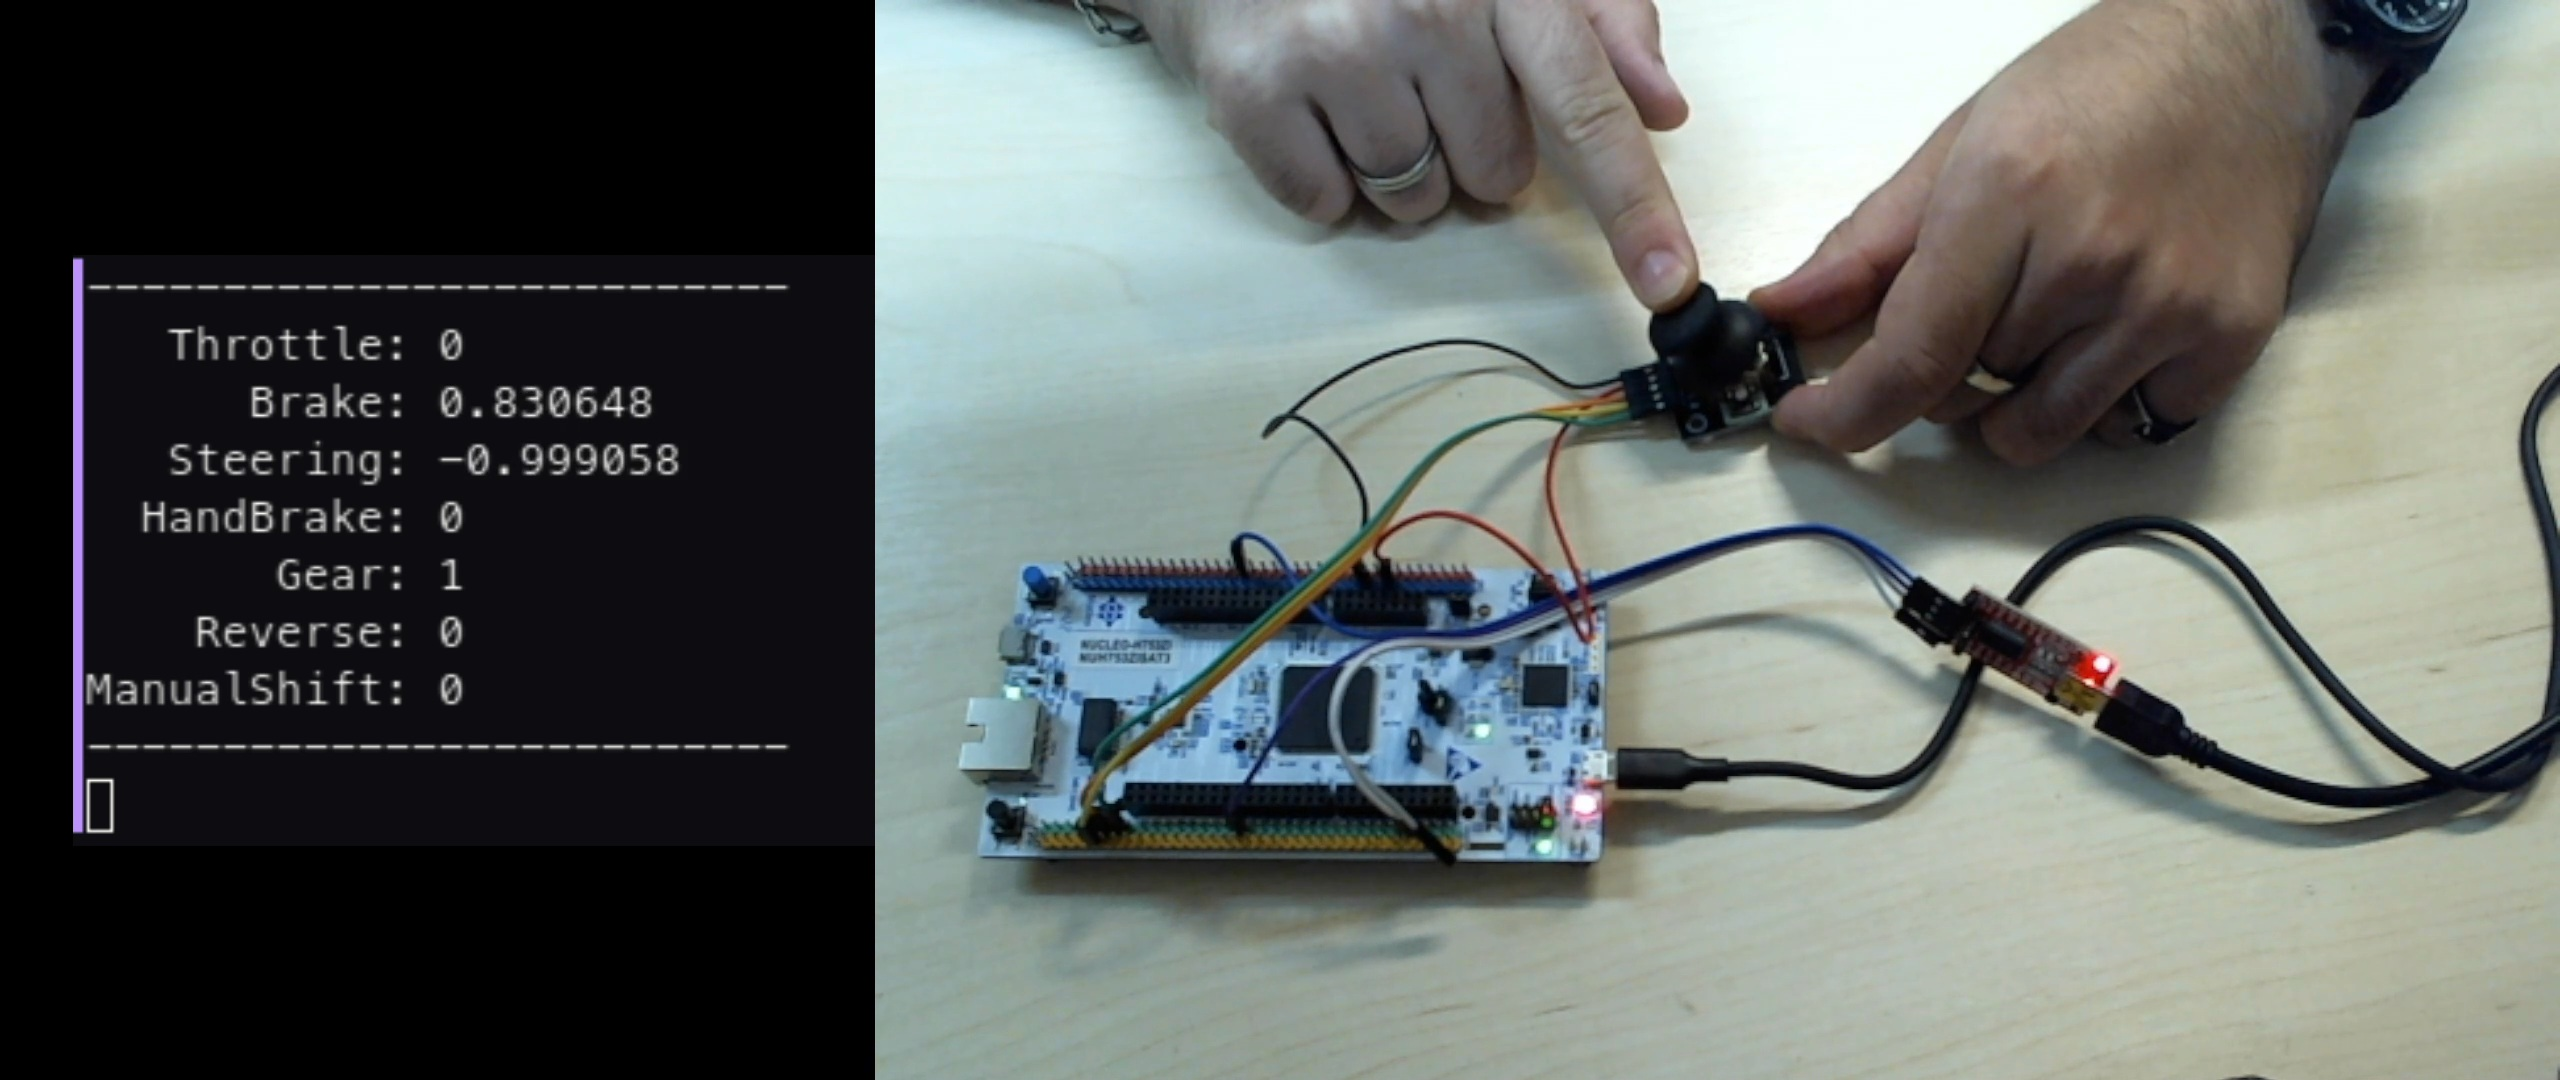
\includegraphics[width=\linewidth]{joyadc}}{TestJoyADC.mp4}
		\caption{Leitura do Joystick pelo \textit{node} \texttt{CarlaSerialBridge}.}
		\label{fig:TestJoyADC}
	\end{figure}
	
\end{frame}       

\begin{frame}{Interrupção JoySW}
	
	\begin{figure}[H]
		\centering
		\movie[width=\textwidth,height=0.422\textwidth,poster,autostart,loop]{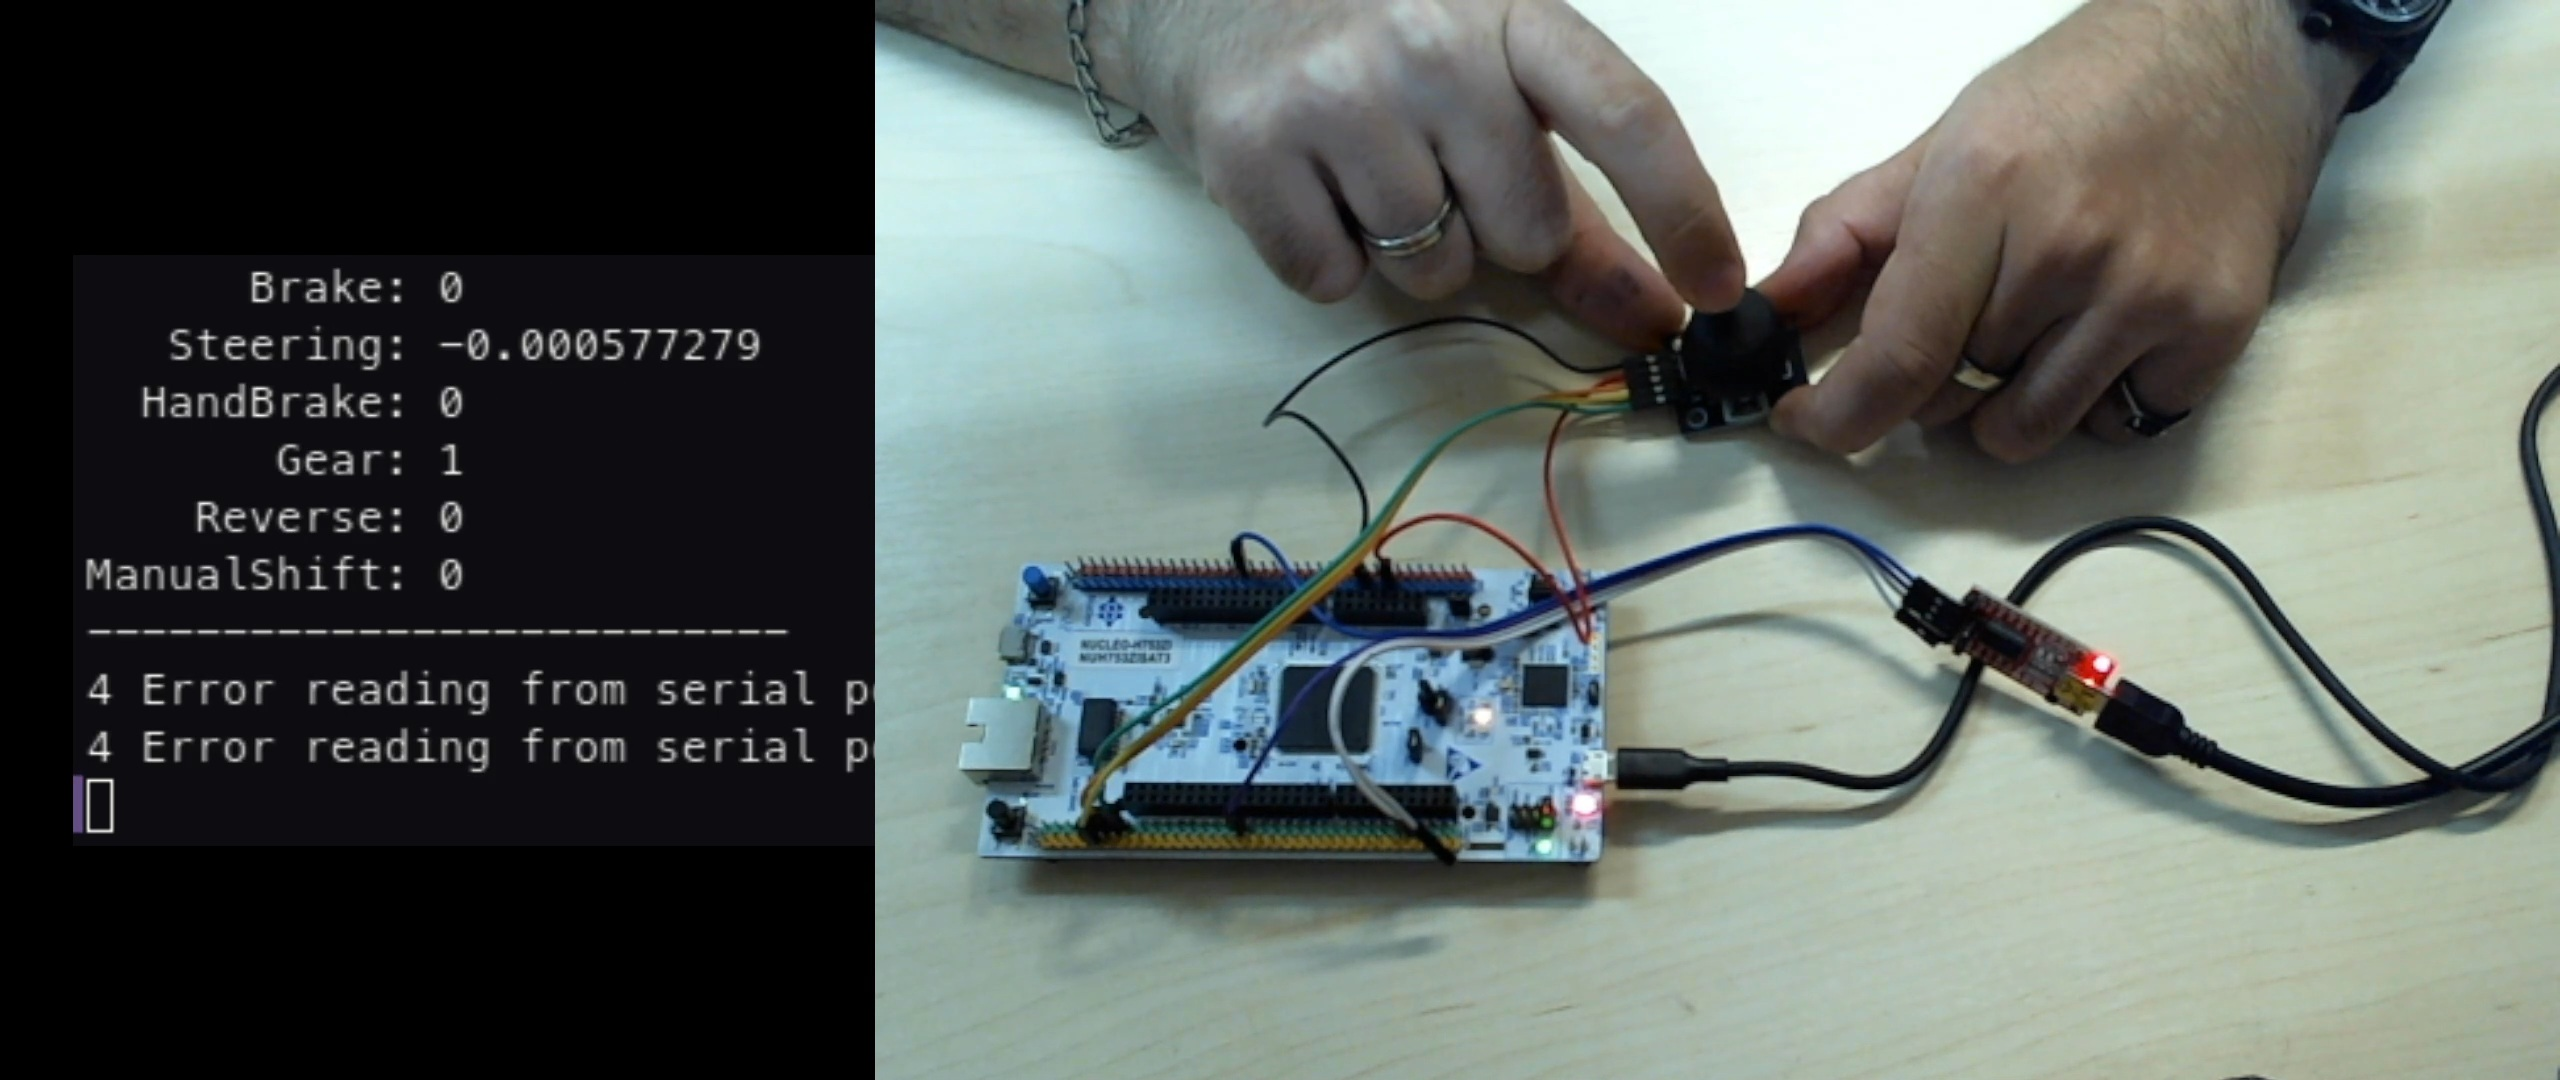
\includegraphics[width=\linewidth]{joysw}}{TestJoySW.mp4}
		\caption{Troca de modo de condução pela interrupção EXTI JoySW.}
		\label{fig:TestJoySW}
	\end{figure}



\end{frame}


\begin{frame}{Modo de operação manual}
	
	\begin{figure}[H]
		\centering
		\movie[width=0.85\textwidth,height=0.478\textwidth,poster,autostart,loop]{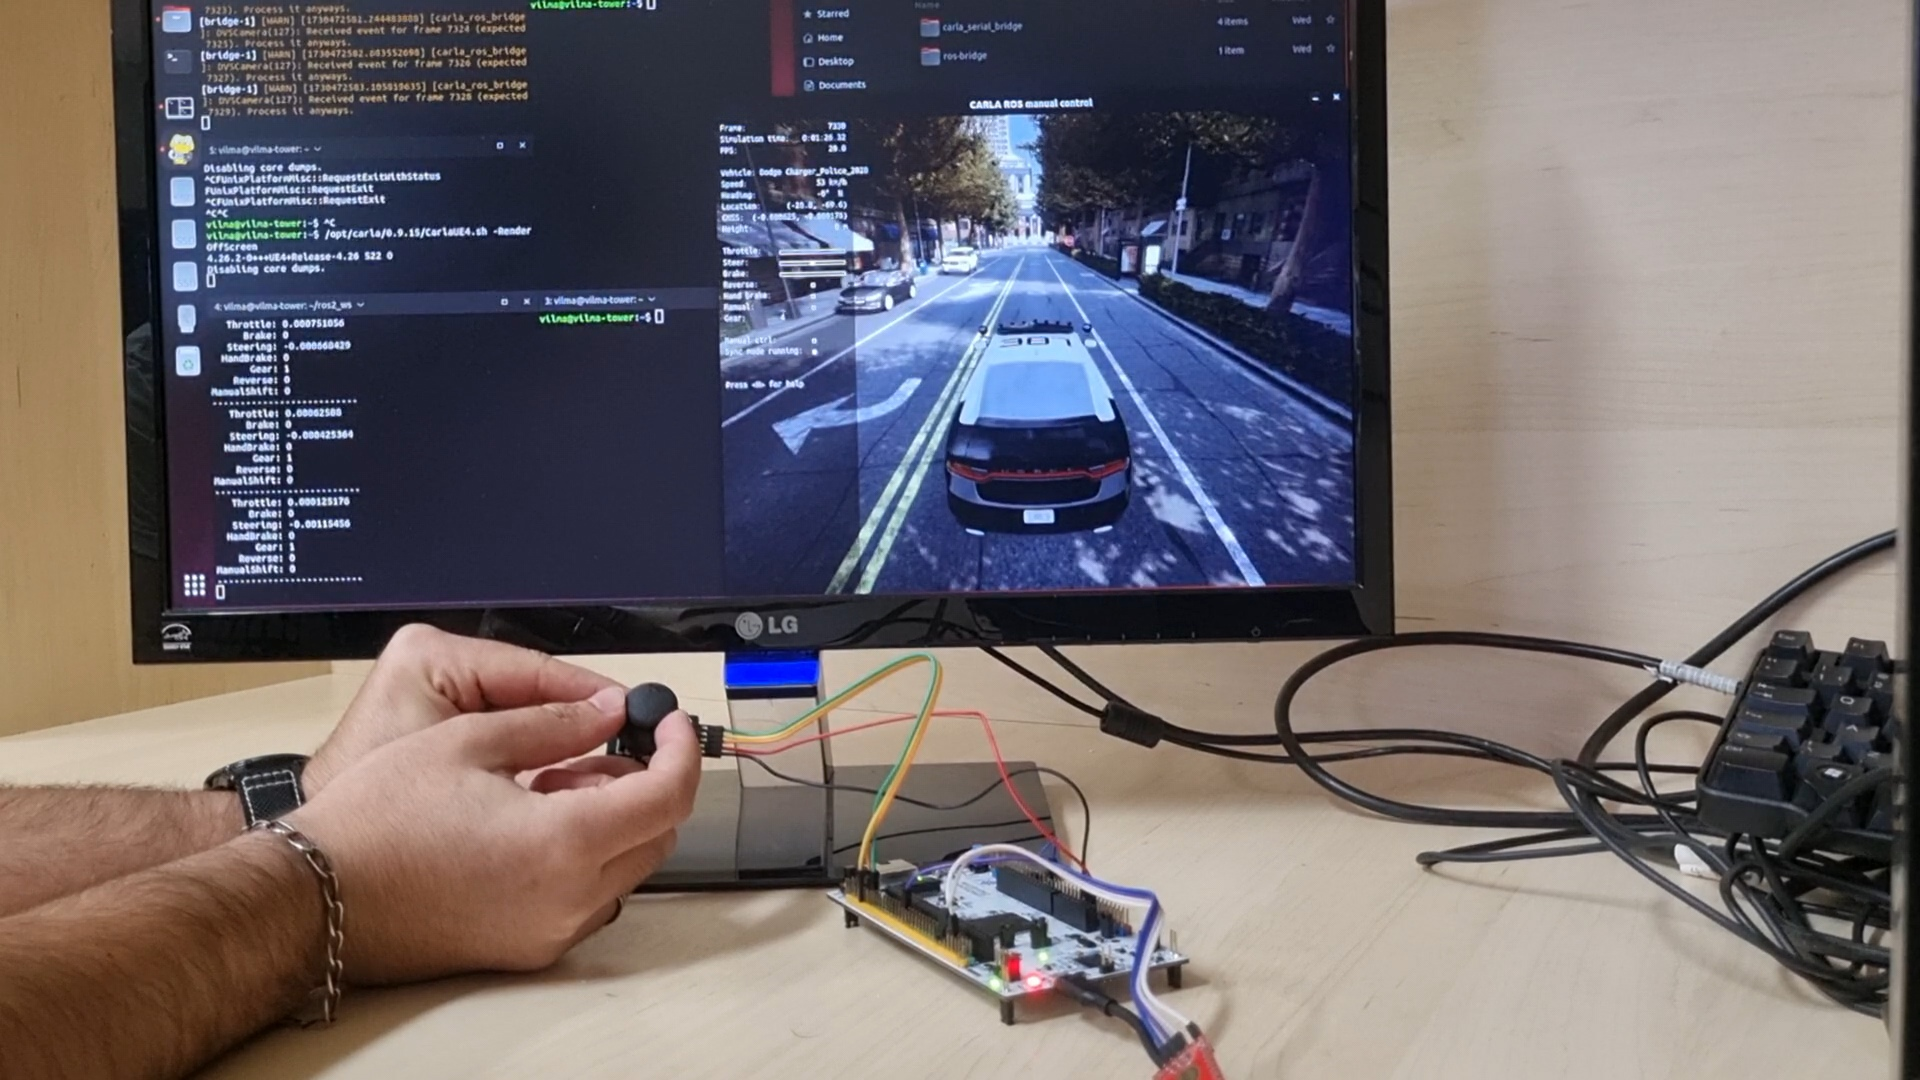
\includegraphics[width=0.85\linewidth]{controle_manual}}{controle_manual.mp4}
		\caption{Validação da comunicação serial com o simulador e controle manual.}
		\label{fig:controle_manual}
	\end{figure}
	
	
\end{frame}


\begin{frame}{micro-ROS \textit{Vehicle Interface}}

	\begin{figure}[H]
		\centering
		\includegraphics[width=0.85\linewidth]{rosgraph}
		\caption{Diagrama de \textit{nodes} e \textit{topics} para a \textit{vehicle interface} construída.}
		\label{fig:rosgraph}
	\end{figure}

\end{frame}


\begin{frame}{ROS}

\begin{figure}[H]
	\centering
	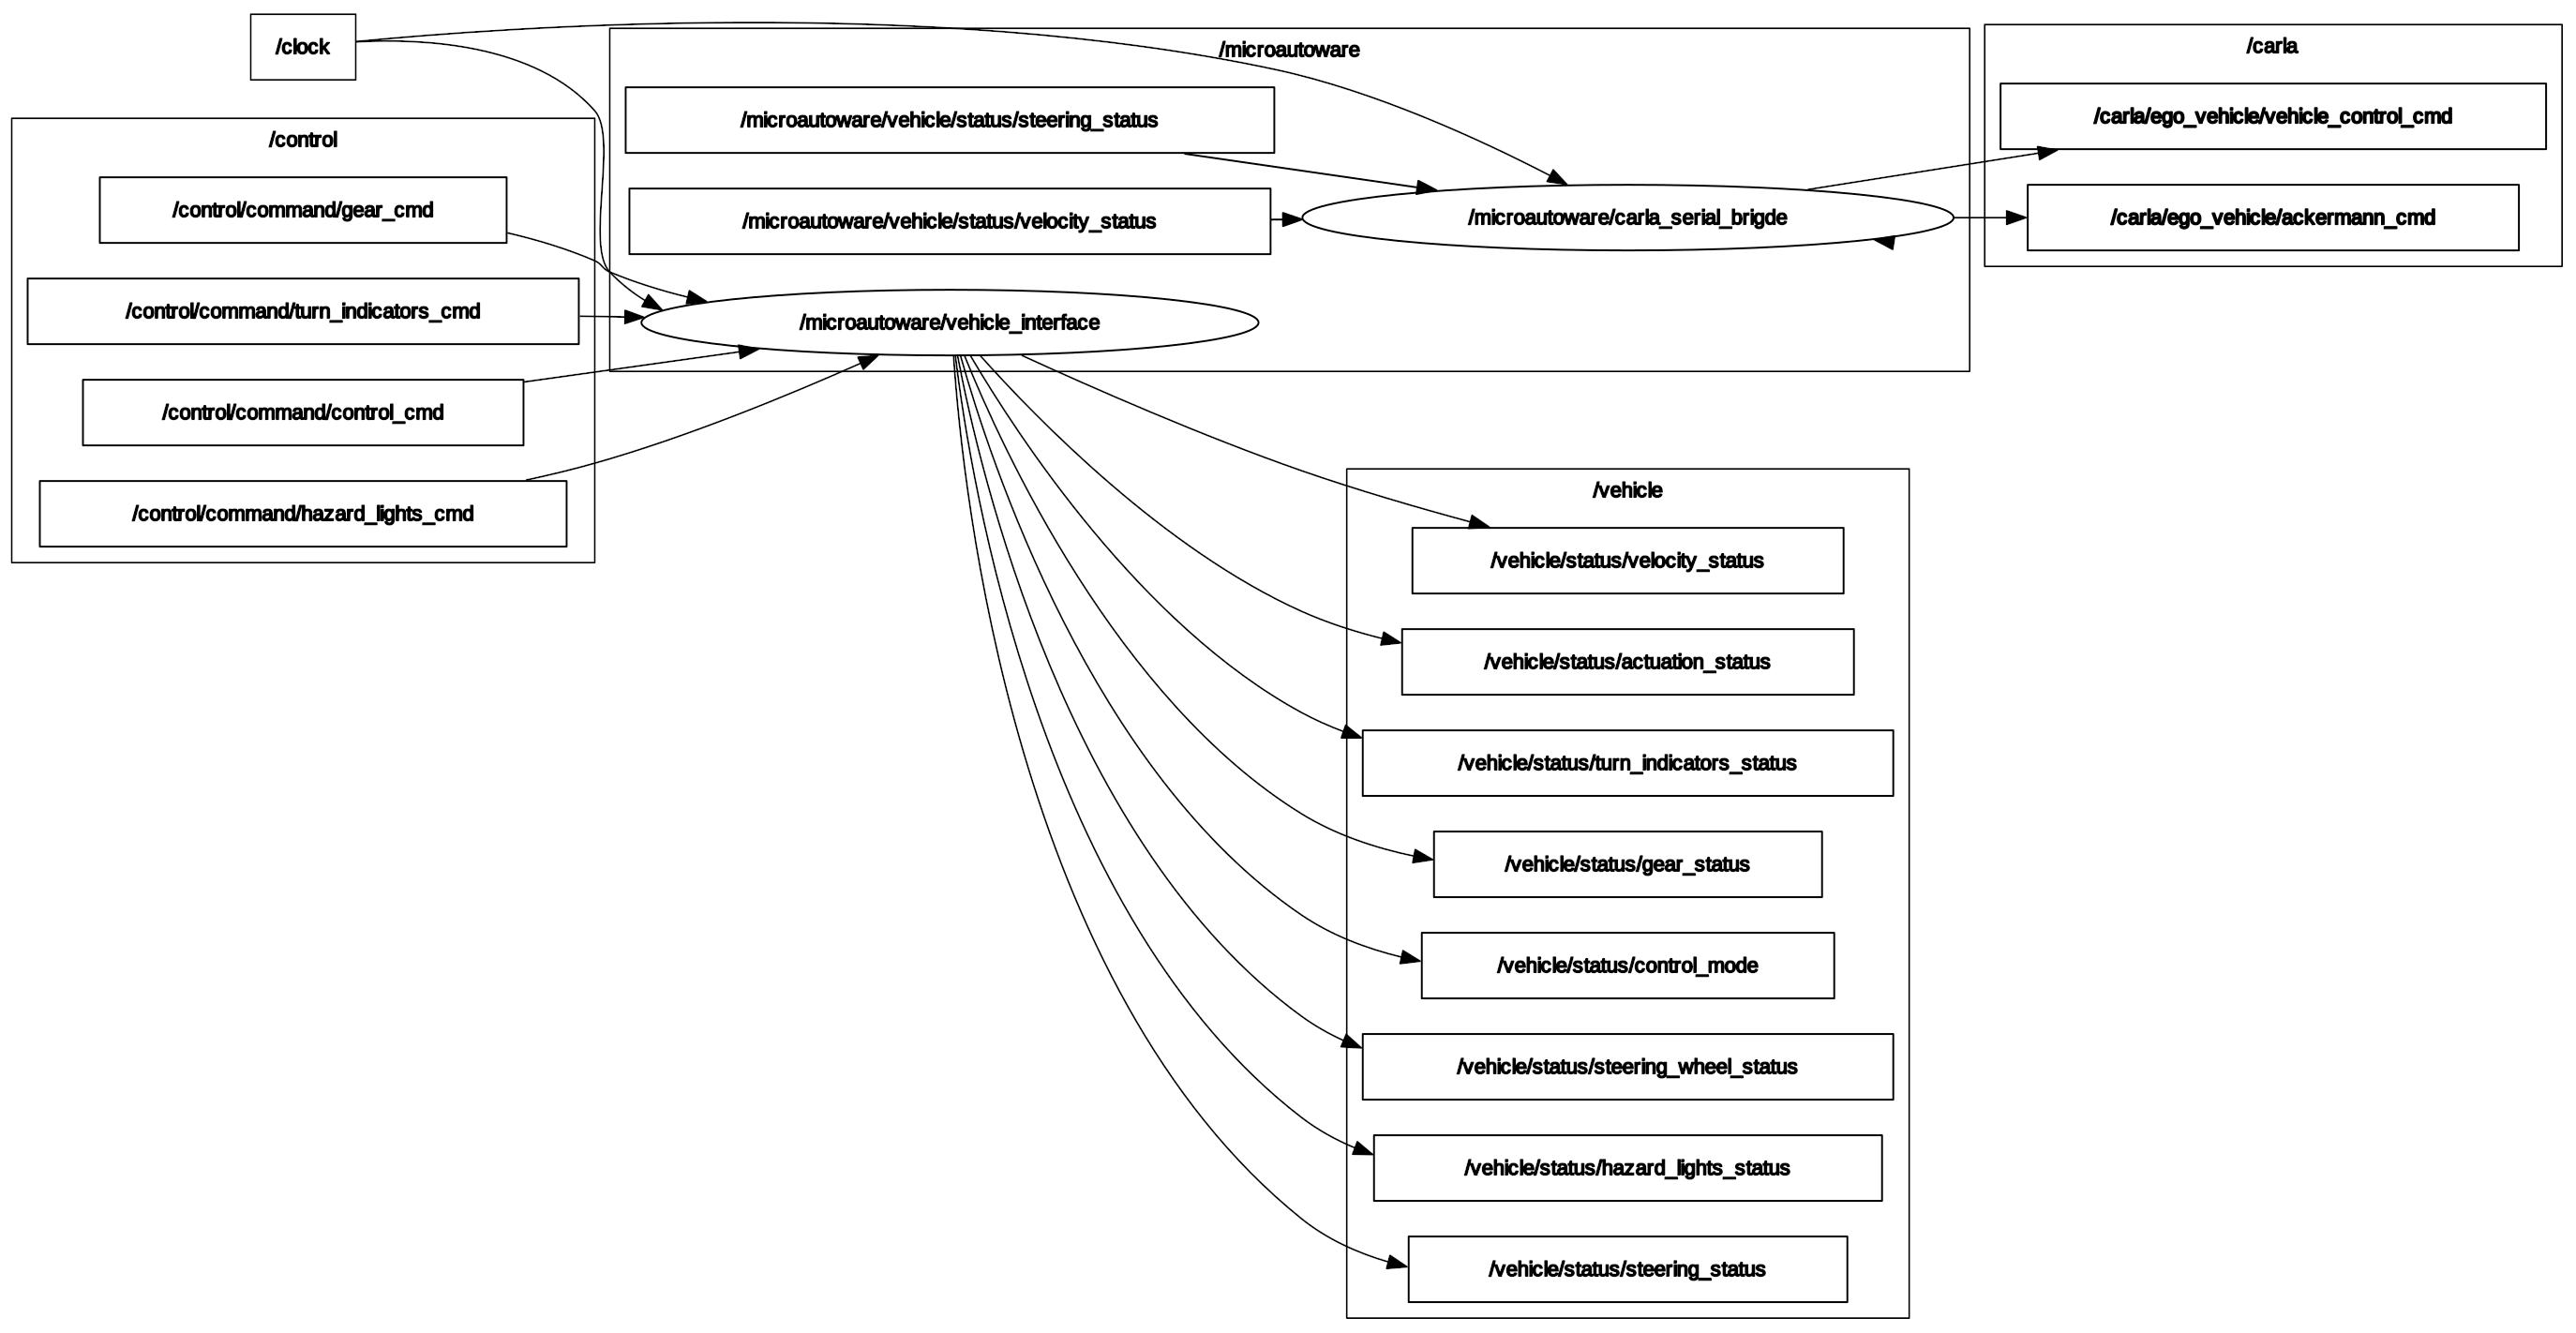
\includegraphics[width=0.95\linewidth]{rosgraph_2}
	\caption{Diagrama de \textit{nodes} e \textit{topics} da arquitetura HIL.}
	\label{fig:rosgraph_2}
\end{figure}

\end{frame}

\begin{frame}{ROS: micro-ROS \textit{Vehicle Interface} }
	
\begin{figure}[H]
	\centering
	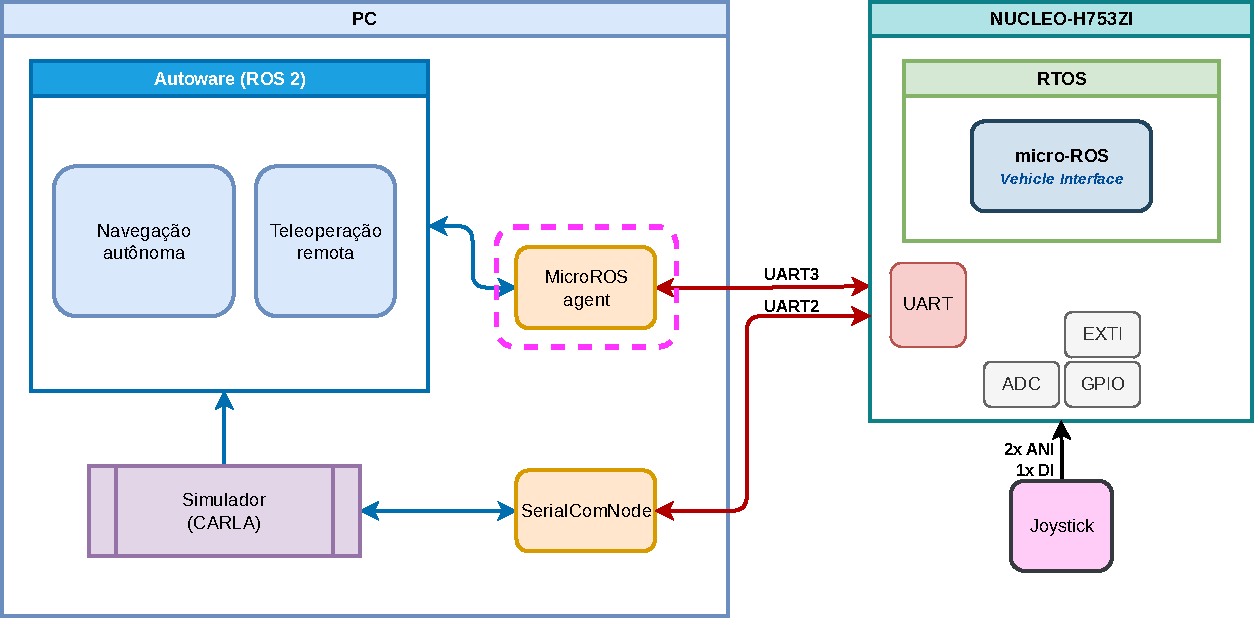
\includegraphics[width=0.9\linewidth]{micro_ros_nodes_scope}
	\caption{Diagrama de blocos -- micro-ros.}
	\label{fig:micro_ros_nodes_scope}
\end{figure}	
	
\end{frame}


\begin{frame}{ROS: micro-ROS \textit{Vehicle Interface} }

\begin{figure}[H]
	\centering
	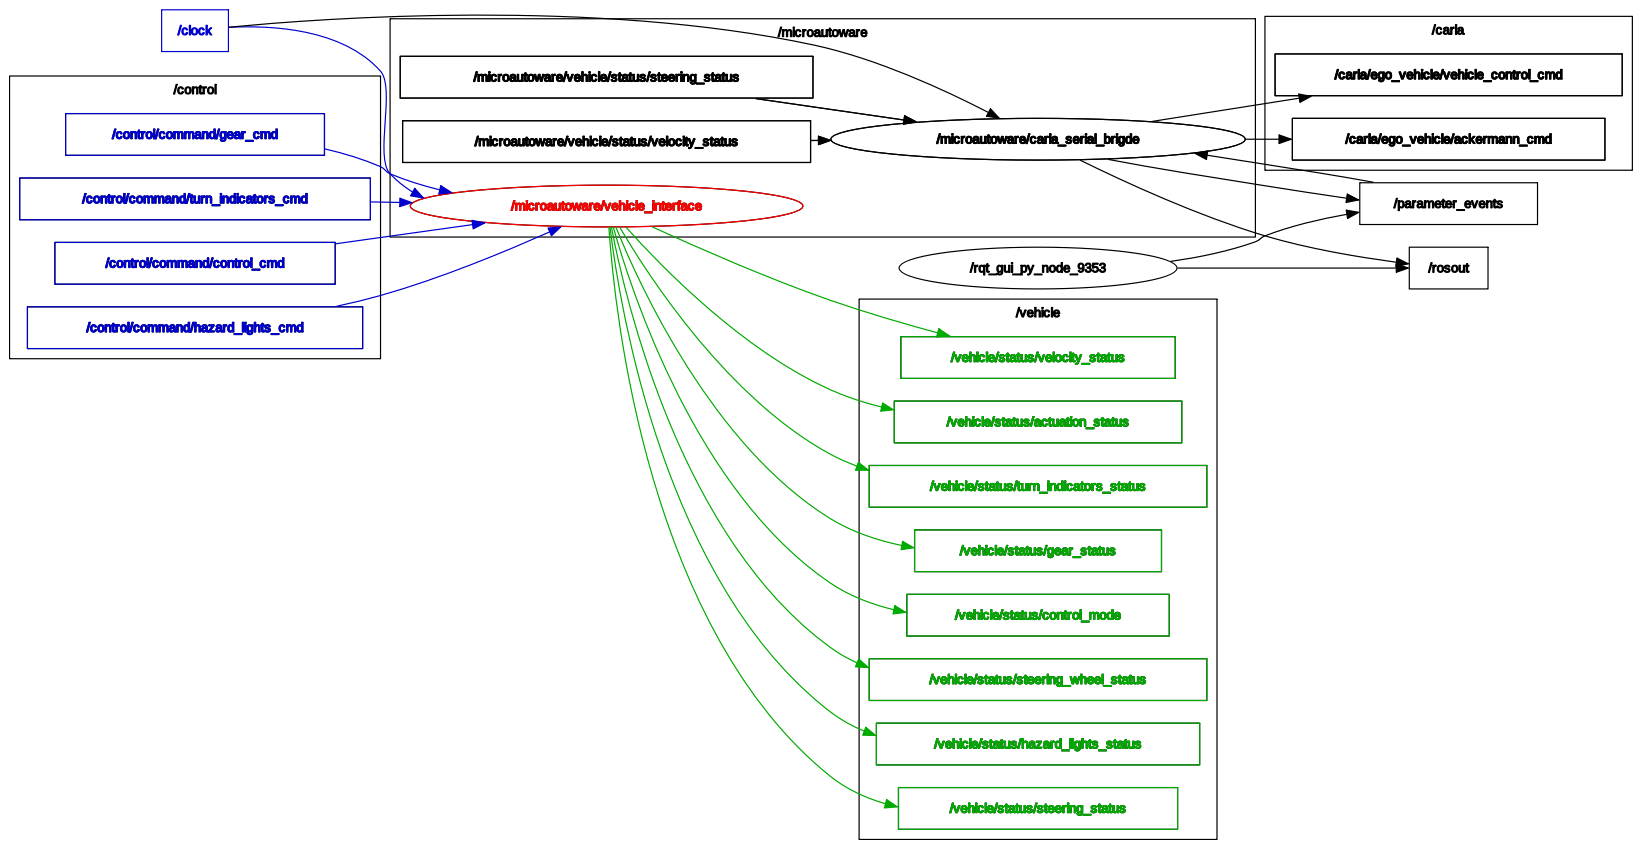
\includegraphics[width=0.95\linewidth]{ros_graph_vi}
	\caption{Diagrama de \textit{nodes} e \textit{topics} da arquitetura HIL (\textit{vehicle interface}).}
	\label{fig:ros_graph_vi}
\end{figure}

\end{frame}

\begin{frame}{ROS: CARLA-Serial-Bridge}

\begin{figure}[H]
	\centering
	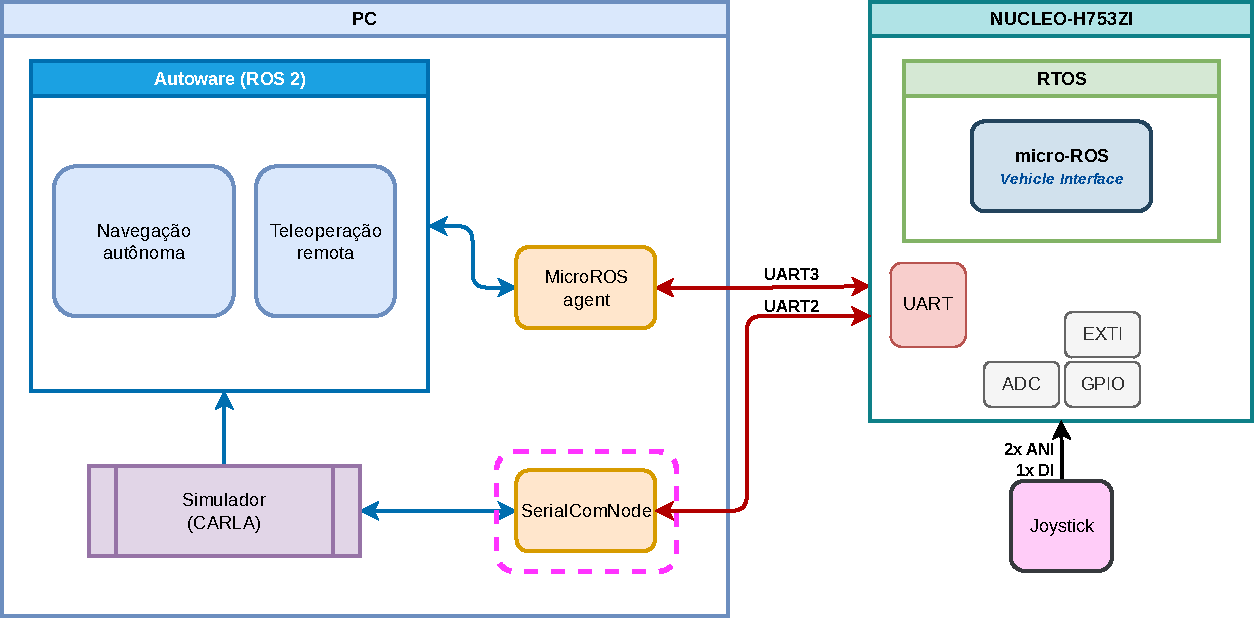
\includegraphics[width=0.9\linewidth]{carla_bridge_nodes_scope}
	\caption{Diagrama de blocos -- CARLA-Serial-Bridge.}
	\label{fig:carla_bridge_nodes_scope}
\end{figure}	

\end{frame}



\begin{frame}{ROS: CARLA-Serial-Bridge}

\begin{figure}[H]
	\centering
	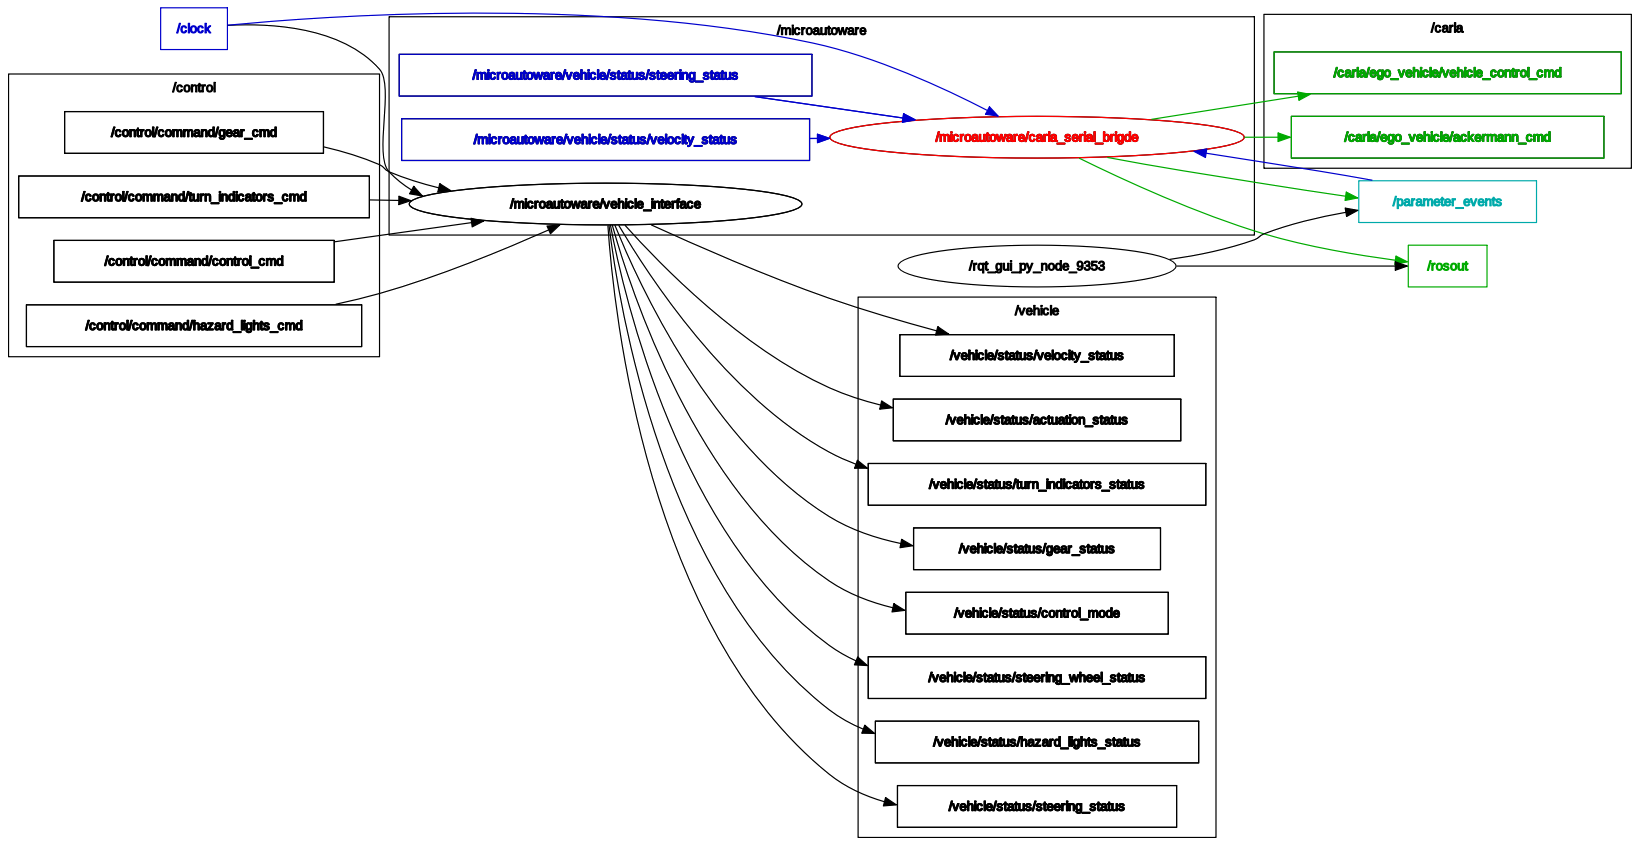
\includegraphics[width=0.95\linewidth]{ros_graph_serial}
	\caption{Diagrama de \textit{nodes} e \textit{topics} da arquitetura HIL (ponte serial com o CARLA).}
	\label{fig:ros_graph_serial}
\end{figure}

\end{frame}


\begin{frame}{Teste do fluxo de dados ROS $\times$ micro-ROS}

\begin{figure}[H]
	\centering
	\movie[width=\textwidth,height=0.422\textwidth,poster,autostart,loop]{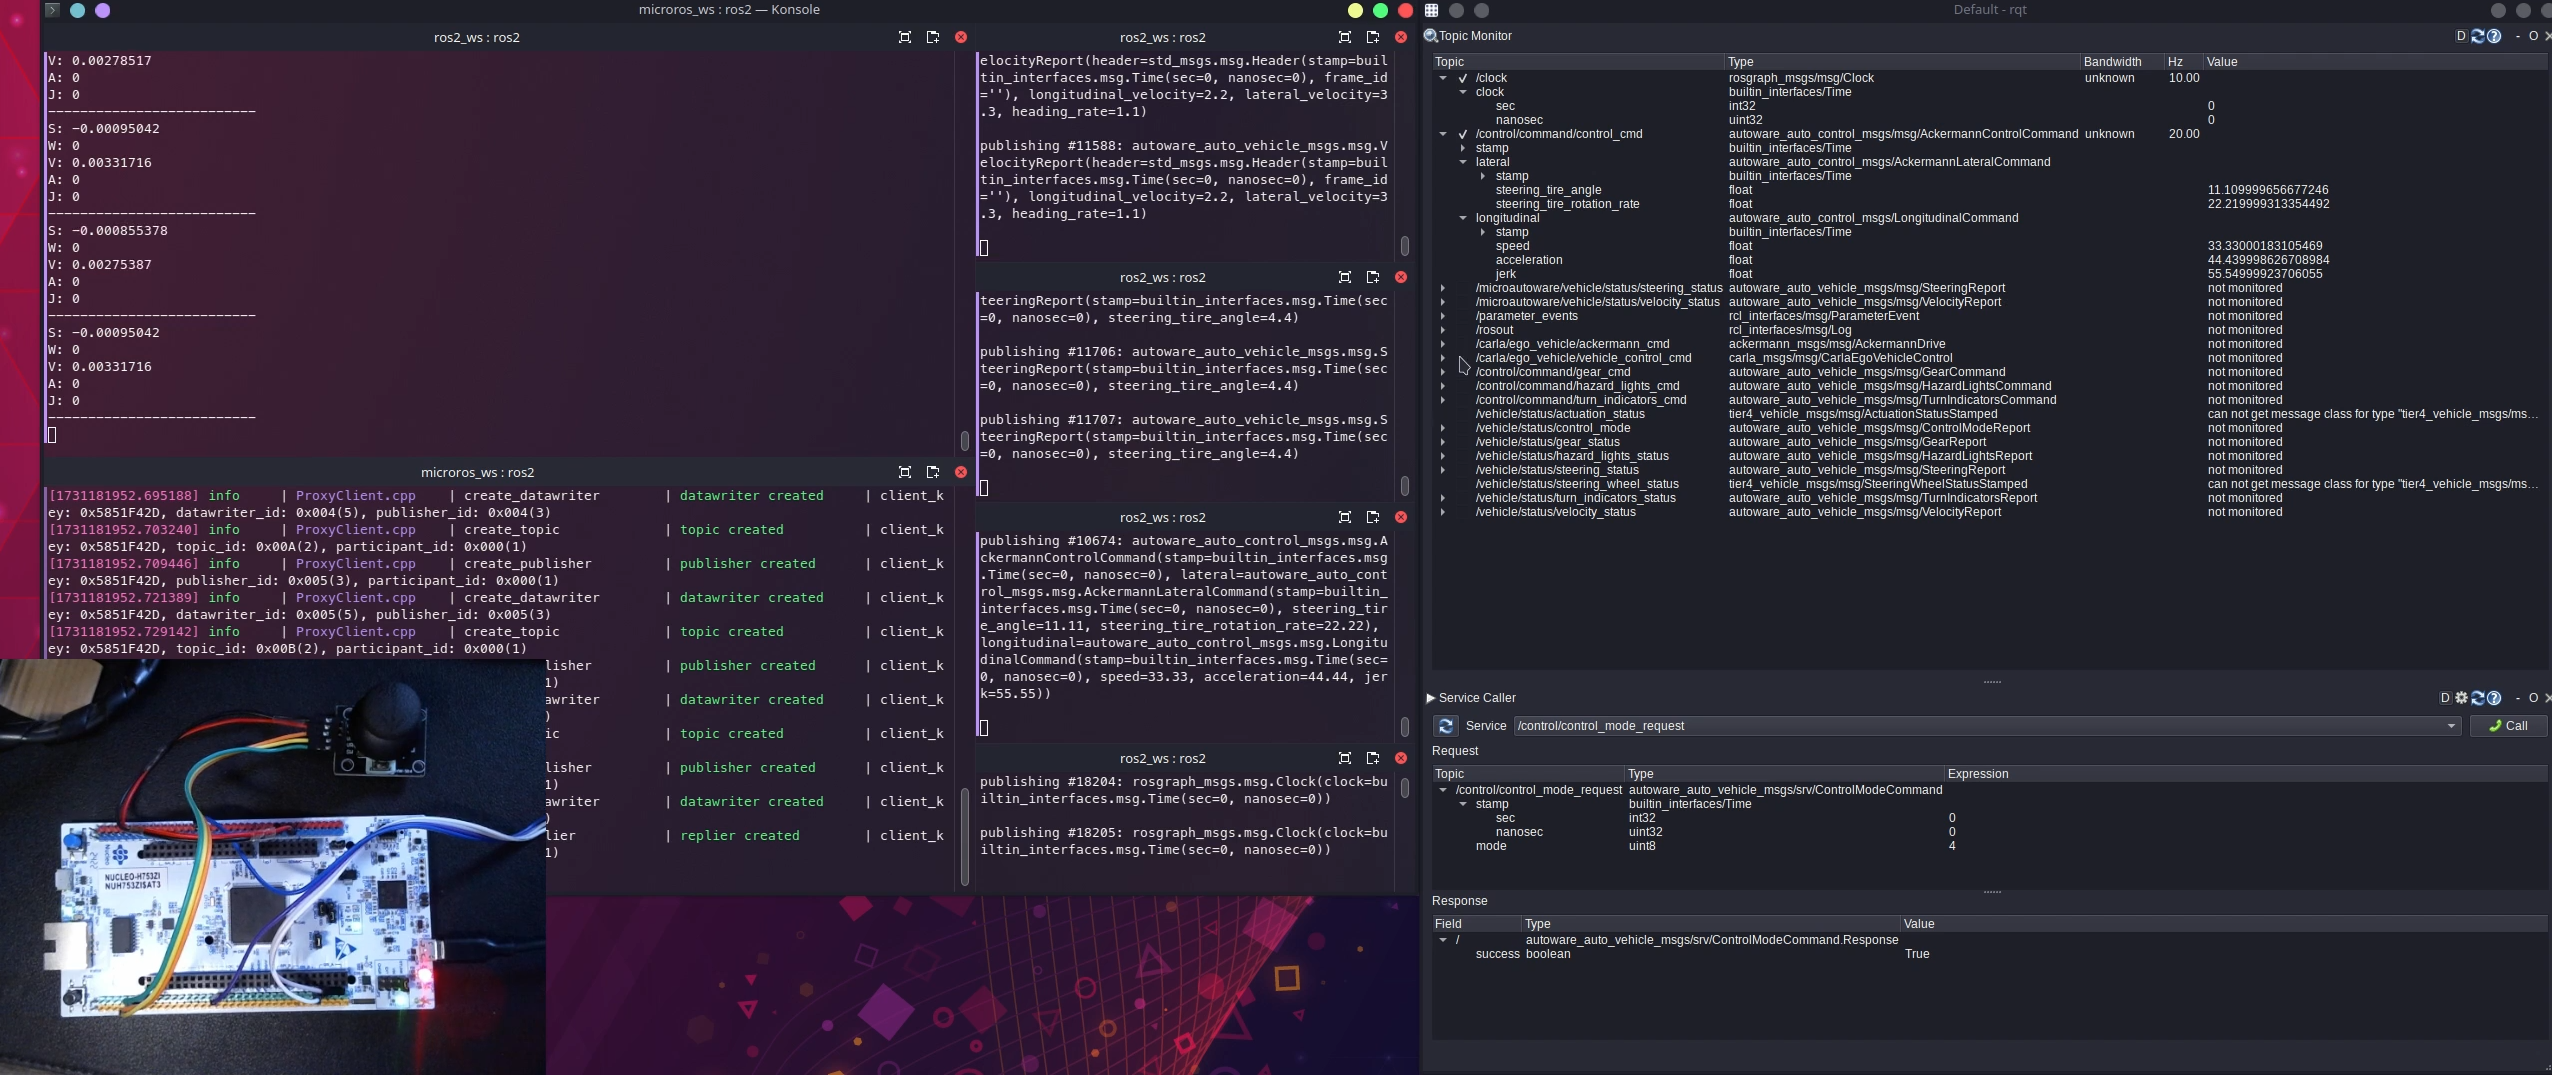
\includegraphics[width=\linewidth]{teste_micro-ros}}{teste_micro-ros.mp4}
	\caption{Validação da comunicação dos tópicos e serviços no micro-ROS.}
	\label{fig:teste_micro}
\end{figure}

\end{frame}


\begin{frame}{Teste \texttt{Carla-Autoware-Bridge}}

\begin{figure}[H]
	\centering
	\movie[width=0.85\textwidth,height=0.478\textwidth,poster,autostart,loop]{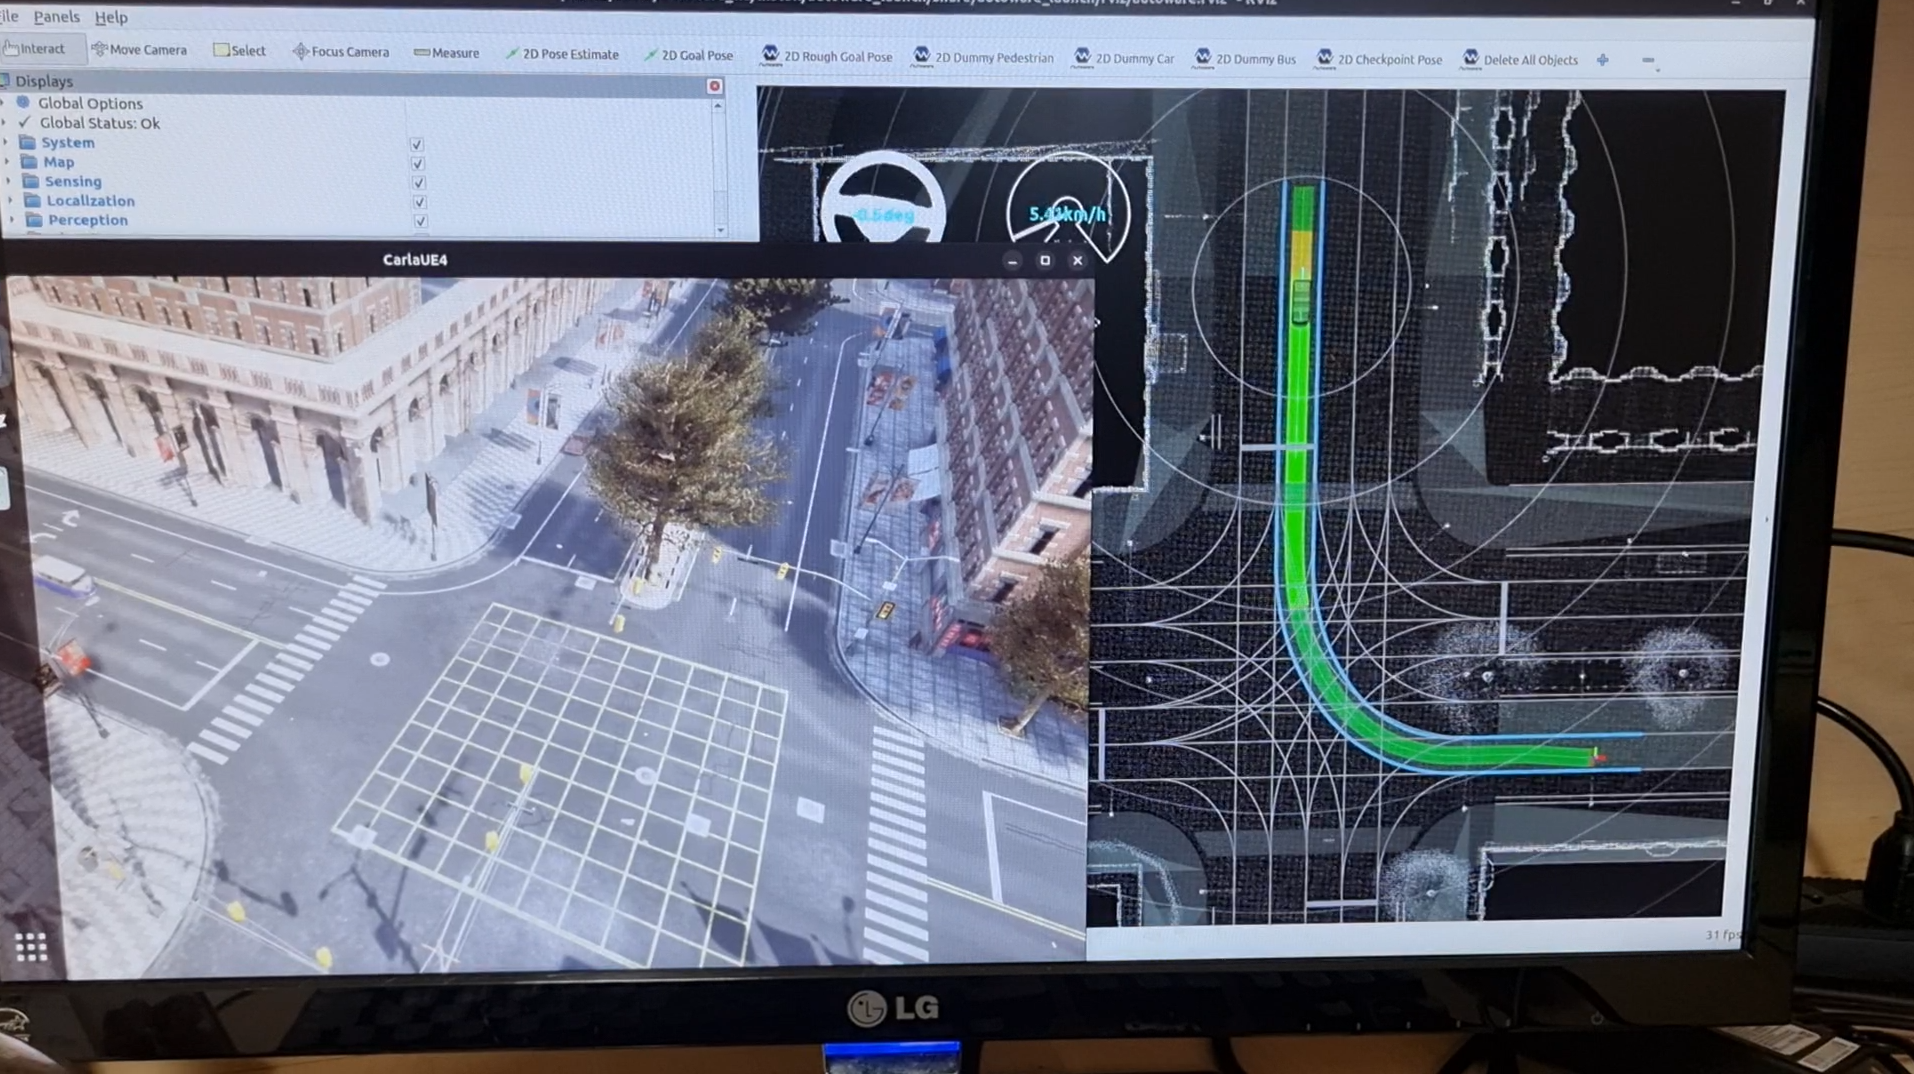
\includegraphics[width=0.85\linewidth]{teste0_autoware}}{teste0_autoware.mp4}
	\caption{Validação do Autoware em modo autônomo.}
	\label{fig:teste0autoware}
\end{figure}


\end{frame}

\section{Problemas encontrados}

\begin{frame}{Problemas encontrados}
	
	\begin{columns}
		
		\begin{column}{0.5\textwidth}
			
			\begin{block}{Problemas diagnósticados}
				
				\begin{itemize}
					\item Perda de ThreadFlags;
					\begin{itemize}
						\item Leitura de \textit{flags} com \texttt{osThreadFlagGet()} antes de \texttt{osThreadFlagWait()}.
						
					\end{itemize}
					\item \textit{Bounce} no botão JoySW.
					\begin{itemize}
						\item \textit{Debounce} em \textit{software} por meio de bloqueio por 1000 \textit{ticks}.
						
					\end{itemize}
					
				\end{itemize}
				
			\end{block}
			
		\end{column}
		
		\begin{column}{0.5\textwidth}
			
			\begin{block}{Problemas à serem verificados}
				
				\begin{itemize}
					\item Escolha dos \textit{timeouts};
					\item Escolha das taxas de envio de dados;
					\begin{itemize}
						\item CARLA $\leftrightarrow$ microAutoware $\leftrightarrow$ Autoware.
						
					\end{itemize}
					\item Política de entrada e saída do modo de emergência.
				\end{itemize}
				
			\end{block}
			
		\end{column}
		
	\end{columns}
	
\end{frame}


\section{Cronograma}

\begin{frame}{Cronograma}
	
	
\begin{table}
	\centering
	\small{
		\begin{tabular}{|b|b|b|b|b|b|b|b|b|b|}
			\hline
			\textbf{Atividade/Semana} & 1 \cellcolor{lightgray} & \textbf{2} \cellcolor{lightgray} & 3 \cellcolor{lightgray} & \textbf{4} \cellcolor{lightgray} & 5 \cellcolor{lightgray} & 6 \cellcolor{lightgray} & \textbf{7} & 8 & \textbf{9} \\
			\hline
			Proposta do projeto  & \cellcolor{unifeiblue} &  &  &  &  &  &  &  &  \\
			\hline
			Projeto de \textit{hardware} e \textit{software}  &  & \cellcolor{unifeiblue} & \cellcolor{unifeiblue} &  &  &  &  &  &  \\
			\hline
			Integração do STM com o micro-ROS  &  & \cellcolor{unifeiblue} &  &  &  &  &  &  &  \\
			\hline
			Integração do micro-ROS com o Autoware  &  &  & \cellcolor{unifeiblue} & \cellcolor{unifeiblue} & \cellcolor{unifeiblue} &  &  &  &  \\
			\hline
			Implementação das tarefas do sistema embarcado  &  &  &  & \cellcolor{unifeiblue} & \cellcolor{unifeiblue} & \cellcolor{unifeiblue} & \cellcolor{unifeiblue} &  &  \\
			\hline
			Construção do ambiente de testes  &  &  &  &  & \cellcolor{unifeiblue} & \cellcolor{unifeiblue} & \cellcolor{unifeiblue} &  &  \\
			\hline
			Realização dos testes  &  &  &  &  &  &  & \cellcolor{unifeiblue} & \cellcolor{unifeiblue} & \cellcolor{unifeiblue} \\
			\hline
			Escrita do relatório  &   & \cellcolor{unifeiblue} & \cellcolor{unifeiblue} & \cellcolor{unifeiblue} & \cellcolor{unifeiblue} & \cellcolor{unifeiblue} & \cellcolor{unifeiblue} & \cellcolor{unifeiblue} & \cellcolor{unifeiblue} \\
			\hline
		\end{tabular}
	}
	\caption{Cronograma de atividades.}
	\label{tab:crono}
\end{table}
	
	\begin{itemize}
		\small
		\item {\color{gray}\textbf{Semana 2:} Apresentação Etapa 1}
		\item {\color{gray}\textbf{Semana 4:} Apresentação Etapa 2}
		\item \textbf{Semana 7:} Apresentação Etapa 3
		\item \textbf{Semana 9:} Apresentação Final
	\end{itemize}
	
\end{frame}


% -------------------------------------------------
%               Bibliografia.
%--------------------------------------------------
%\section{Referências bibliográficas}
%\begin{frame}{Referências bibliográficas}
%   %\bibliographystyle{acm}
%   \bibliography{bibliografia.bib}
%\end{frame}



\begin{frame}{}
	
	\begin{block}{}
		
		\centering
		\Huge{Obrigado!}
		
		\LARGE
		
		\vspace{5mm}
		
		Dúvidas?
		
	\end{block}
	
	\vspace{4mm}
	
	\begin{figure}[H]
		\centering
		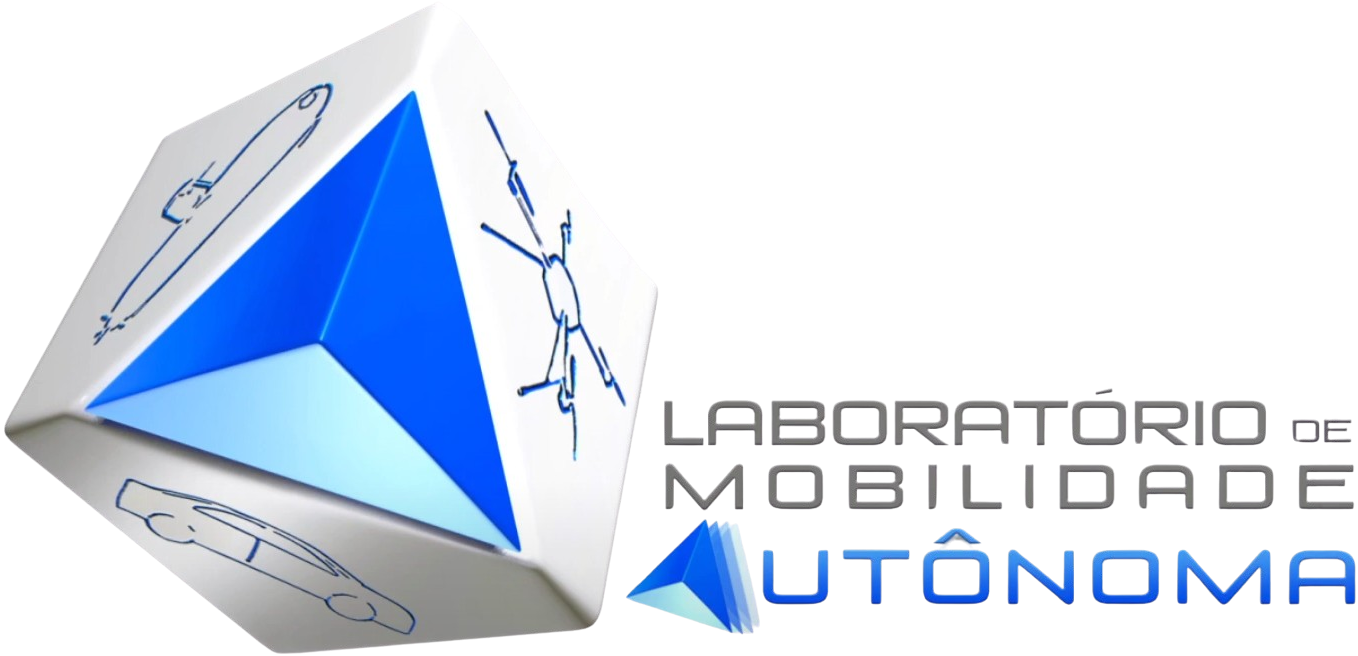
\includegraphics[width=0.5\linewidth]{img/core/Logo_LMA.png}
	\end{figure}
	
\end{frame}

\end{document}
